\documentclass[11pt, a4paper]{article}
\usepackage[utf8]{inputenc}
\usepackage[ngerman]{babel}
\usepackage[T1]{fontenc}
\usepackage{amsmath}
\usepackage{amsfonts}
\usepackage{amssymb}
\usepackage{hyperref}
\usepackage{enumitem}
\usepackage{geometry}
\usepackage{adjustbox}
\usepackage{graphicx}
\graphicspath{{Images/}}


\title{Software Engineering}
\author{Zusammenfassung}
\date{SoSe 2024}

\begin{document}
\maketitle

\tableofcontents
\newpage


% --- START DES EIGENTLICHEN INHALTS -------------------------------------------------


\section{Einführung} % --- Einführung ------------------------------------------------------------------------------------

\subsection{Ziele des Software Engineering}

\begin{enumerate}
    \item \textbf{Qualität}:
    \begin{itemize}
        \item Zuverlässigkeit
        \item Wartbarkeit
        \item Benutzerfreundlichkeit
        \item Performanz
        \item Effizienz
    \end{itemize}

    \item \textbf{Kosten}:
    \begin{itemize}
        \item Entwicklungskosten
        \item Wartungskosten
        \item Vertriebskosten
    \end{itemize}

    \item \textbf{Zeit}:
    \begin{itemize}
        \item Verkürzung der Entwicklungszeit durch mehr Personal
        \item Spezialisten und motivierte Teams
    \end{itemize}

    \item \textbf{Wirtschaftlichkeit}:
    \begin{itemize}
        \item Umsatz und Kosteneinsparung durch effiziente Softwarelösungen
    \end{itemize}
\end{enumerate}

\newpage

\section{Ethik} % --- Ethik ------------------------------------------------------------------------------------

\subsection{Internationale Organisationen}

\begin{itemize}
    \item ACM(Association for Computing Machinery)
    \item IEEE (Institute of Electrical and Electronic Engineers)
    \item British Computer Society
\end{itemize}

“Software Engineering Code of Ethics and Professional Practice”

\footnotesize \url{https://ethics.acm.org/code-of-ethics/software-engineering-code/}

\subsection{8 Prinzipien des ACM/IEEE Code of Ethics}

\begin{enumerate}
    \item \textbf{Public}:
    \begin{itemize}
        \item Handeln im öffentlichen Interessen
        \item Volle Verantwortung für seinen Code übernehmen
        \item Genehmigen Sie Software nur, wenn sie sicher ist, die Spezifikationen erfüllt, 
        geeignete Tests besteht und die Lebensqualität nicht beeinträchtigt, 
        die Privatsphäre nicht verletzt und die Umwelt nicht schädigt
    \end{itemize}

    \item \textbf{Client and Employer}:
    \begin{itemize}
        \item Interessen von Kunden und Arbeitgebern wahren
    \end{itemize}

    \item \textbf{Product}:
    \begin{itemize}
        \item Höchste professionelle Standards für Produkte sicherstellen
    \end{itemize}

    \item \textbf{Judgement}:
    \begin{itemize}
        \item Integrität und Unabhängigkeit im beruflichen Urteil bewahren
    \end{itemize}

    \item \textbf{Management}:
    \begin{itemize}
        \item Ethisches Management von Softwareentwicklung und -wartung
    \end{itemize}

    \item \textbf{Profession}:
    \begin{itemize}
        \item Integrität und Reputation des Berufsstandes fördern
    \end{itemize}

    \item \textbf{Colleagues}:
    \begin{itemize}
        \item Fair und unterstützend gegenüber Kollegen sein
    \end{itemize}

    \item \textbf{Self}:
    \begin{itemize}
        \item Lebenslanges Lernen und ethische Praxis fördern
    \end{itemize}
\end{enumerate}

\subsection{Ethikfragen im Software Engineering}

\begin{itemize}
    \item Ist die Verbreitung von Viren/Trojanern ein ethisches Problem?
    \item Ist fehlerhafter Code ein ethisches Problem?
    \item Ist schwer lesbarer Code ein ethisches Problem?
    \item Ist das Unterschätzen der Schwierigkeit eines SW-Projekts ein ethisches Problem?
    \item Ist das Unterschätzen der Kosten eines Softwareprojekts ein ethisches Problem?
    \item Ist es ein ethisches Problem, nicht immer die neuesten Technologien zu nutzen?
\end{itemize}

\newpage

\section{Projektphasen} % --- Projektphasen ------------------------------------------------------------------------------------

\subsection{Wie kommt man zu einem Projekt?}

\begin{figure}[h]
    \centering
    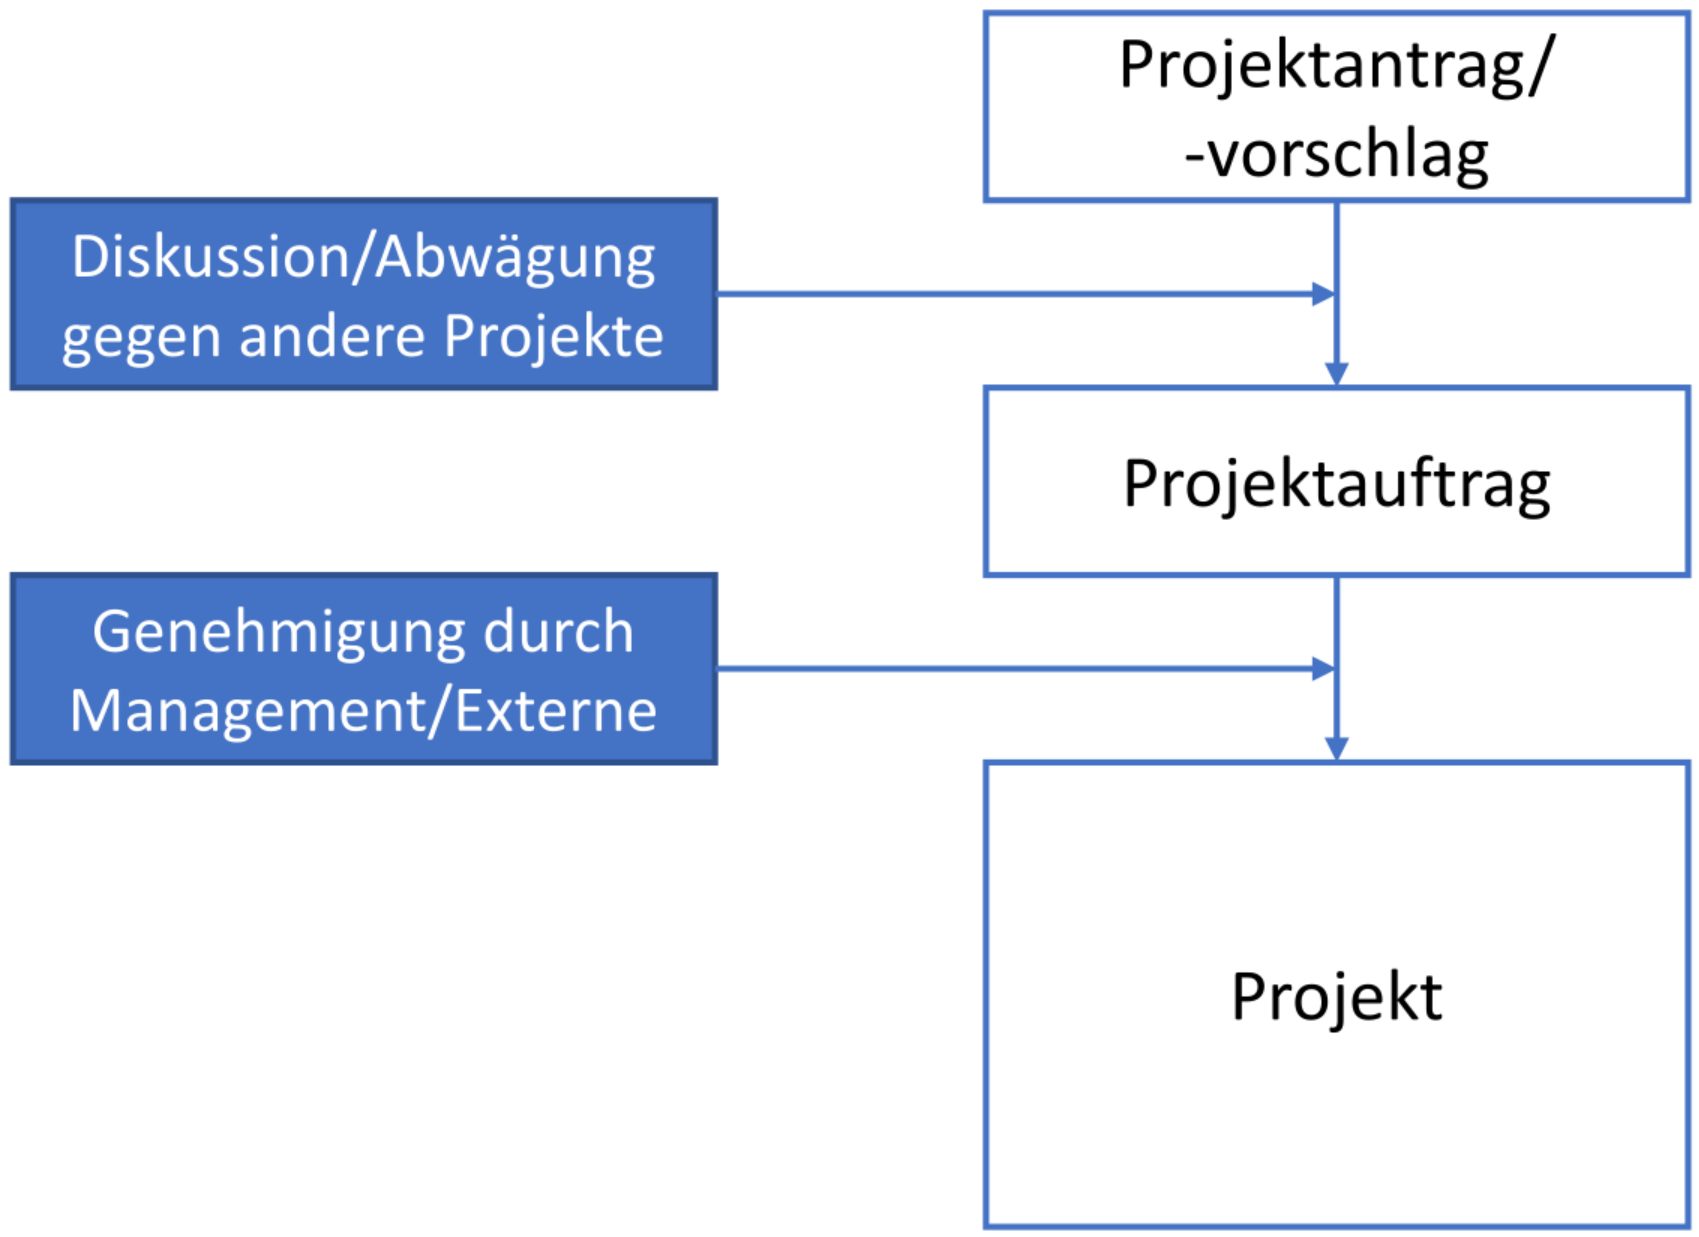
\includegraphics[width=0.75\textwidth]{Projektphasen-00}
    \caption{Projektantrag Ablauf}
    \label{fig:Projektphasen-00}
\end{figure}



\subsubsection{Projektantrag}

\begin{itemize}
    \item \textbf{Ziel:} Darlegung der Projektidee
    \item \textbf{Inhalte:}
    \begin{itemize}
        \item Ausgangslage (Status quo, welches Problem wollen wir lösen?)
        \item Ziele
        \item Kosten/Nutzen
        \item Organisation
    \end{itemize}
    \item \textbf{Ausprägungen:}
    \begin{itemize}
        \item Interne Projekte
        \item öffentlich geförderte Projekte
    \end{itemize}
\end{itemize}

\newpage

\subsubsection{Projektauftrag}

Offizieller Startschuss für das Projekt. Projektauftrag ist das erste Projektdokument. \\
\textbf{!!!Kein Projekt ohne Projektauftrag!!!}

\begin{itemize}
    \item \textbf{Inhalte:} 
    \begin{itemize}
        \item Projektbezeichnung
        \item Auftraggeber
        \item Beginn und Ende
        \item Kurzbeschreibung
        \item Unternehmensbedarf
        \item Ziele
        \item Projektergebnisse
        \item Budget
        \item Projektleiter
        \item Team
        \item Annahmen
        \item Beschränkungen
        \item Terminvorgaben
    \end{itemize}
\end{itemize}

Unternehmen haben sehr unterschiedliche Handhabung im Umgang mit Projektantrag und Projektauftrag. 
Er hängt von Organisationsstruktur und Kultur des Unternehmens ab.
Bei mittelgroßen/großen Unternehmen gibt es normalerweise Vorlagen für den Projektauftrag!

\subsection{Phasen eines Softwareprojekts}

\begin{figure}[h]
    \centering
    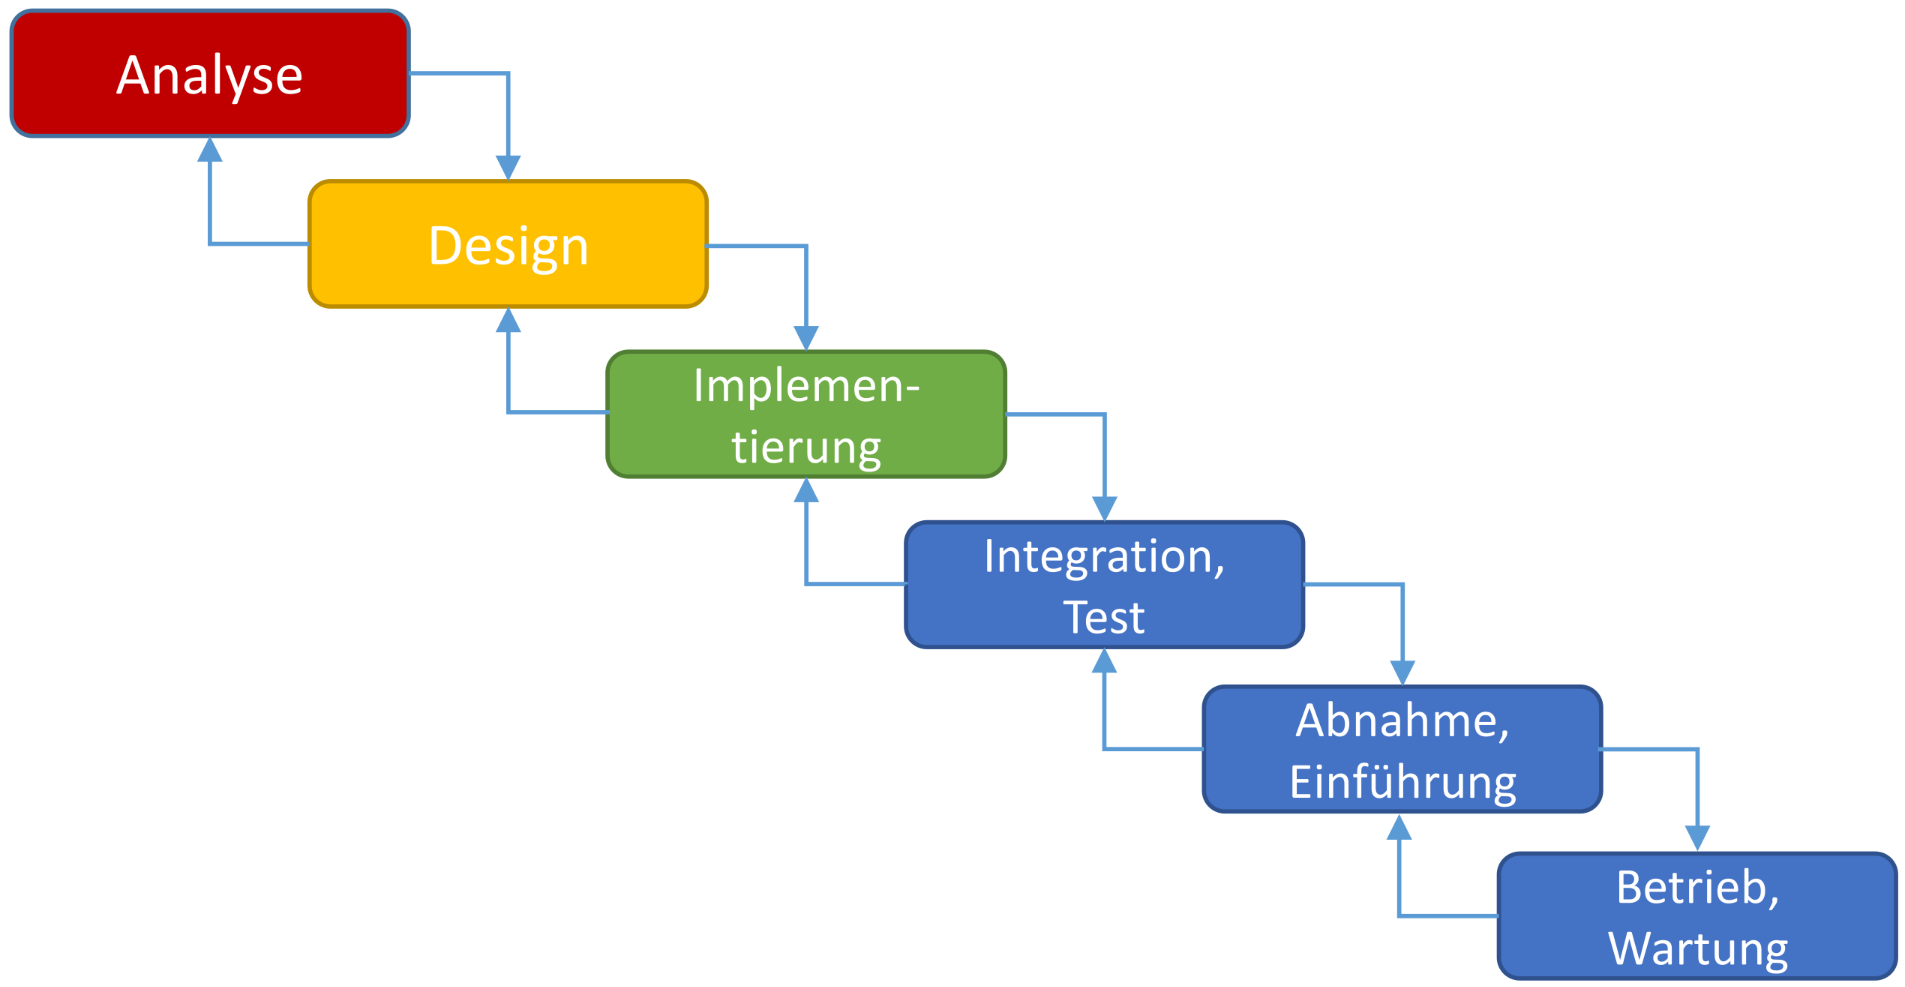
\includegraphics[width=0.75\textwidth]{Projektphasen-01}
    \caption{Projektphasen Ablauf}
    \label{fig:Projektphasen-01}
\end{figure}

\subsubsection*{Analyse}

\begin{itemize}
    \item Aufstellen von Leistungen, Einschränkungen und Zielen des Systems
    \item In Zusammenarbeit mit den Systembenutzern/dem Kunden
    \item Anschließend detailliertere Beschreibung und Definition
    \item Ergebnis dient als Systemspezifikation
\end{itemize}

\subsubsection*{Design (Entwurf)}

\begin{itemize}
    \item Anforderungen werden in Hard- oder Softwaresysteme aufgeteilt
    \item Dazu wird übergeordnete Systemarchitektur festgelegt
    \item Beim Software-Design geht es um Erkennen und Beschreiben:
    \begin{itemize}
        \item Der grundlegenden (abstrakten) Softwaresysteme und
        \item Deren Beziehung zueinander
    \end{itemize}
\end{itemize}

\subsubsection*{Implementierung (und Modultests)}

\begin{itemize}
    \item Umsetzung des Softwareentwurfs durch Programme oder Programmeinheiten
    \item Testen der Module auf Einhaltung Ihrer Spezifikation
\end{itemize}

\subsubsection*{Integration, Test}

\begin{itemize}
    \item Zusammenführung/Integration einzelner Programme oder Programmeinheiten
    \item Test des “Ganzen” auf Einhaltung der Anforderungen
    \item Auslieferung an Kunden
\end{itemize}

\subsubsection*{Abnahme, Einführung}

\begin{itemize}
    \item Abnahmetests in mehreren Stufen
    \begin{itemize}
        \item Technische Tests
        \item Last-/Performancetests
        \item Fachliche Tests
        \item User-Acceptance Tests, …
    \end{itemize}
    \item Auslieferung an den Kunden
    \item Ggf. Anwenderschulungen, Informationsmaßnahmen bis hin zu Marketing für die neue Software
\end{itemize}

\subsubsection*{Betrieb, Wartung}

\begin{itemize}
    \item Längste Phase im Software-Lifecycle
    \item System wird installiert und zur Nutzung freigegeben
    \item Elemente der Wartung:
    \begin{itemize}
        \item Beheben von Fehlern
        \item Verbesserung der Implementierung von Systemeinheiten
        \item Verbesserung des Systems, falls neue Anforderungen entstehen
    \end{itemize}
    \item Teil der Wartung häufig noch in Projektkosten enthalten
    \item Später Wartungsverträge
\end{itemize}

\subsection{Allgemeine Hinweise zu den Projektphasen}

\begin{itemize}
    \item Phasen nicht notwendigerweise sequentiell
    \item Tätigkeiten innerhalb der Phasen erfordern verschiedene Qualifikationen
    \item ABER: nicht immer ist (vollständige) Durchführung aller Phase sinnvoll
    \item Tätigkeiten müssen koordiniert werden → Projektmanagement
    \item Softwareprojekte laufen immer in Teams ab (sowohl innerhalb des Unternehmens als auch mit Kooperationspartnern/Kunden)
\end{itemize}

\textbf{$ \rightarrow $ Kommunikation innerhalb des Teams und zwischen Team und Kunden ist extrem wichtig}

\subsection{Dokumente (Artefakte) pro Phase}

Jede Phase bringt Dokumente (Artefakte) hervor, die Input für die folgende Phase sind

\begin{figure}[h]
    \centering
    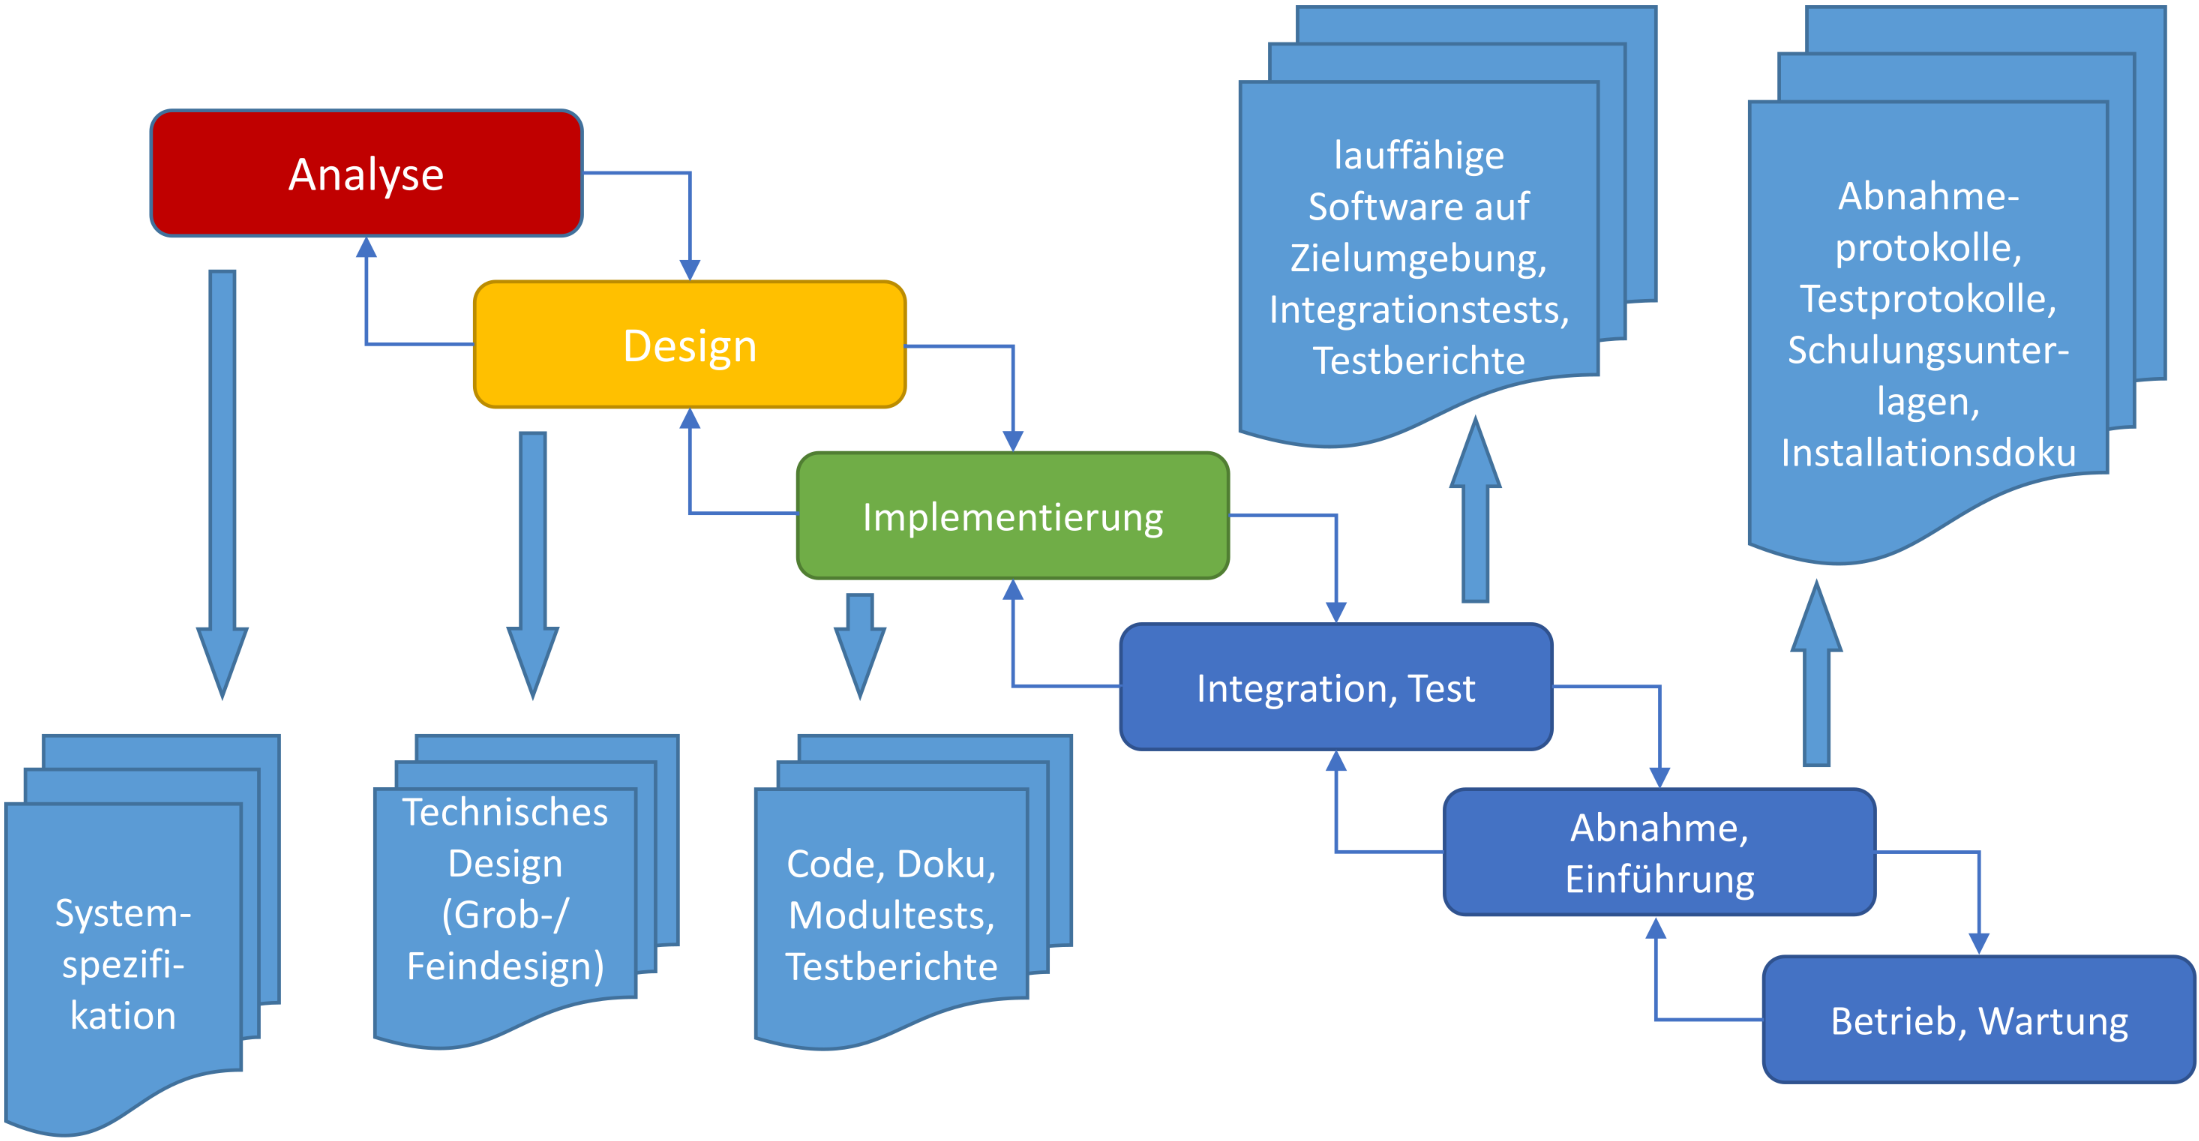
\includegraphics[width=0.75\textwidth]{Projektphasen-02}
    \caption{Dokumente der einzelnen Phasen}
    \label{fig:Projektphasen-02}
\end{figure}

\newpage

\section{Requirements Engineering (Anforderungsanalyse)} % --- Requirements Engineering ------------------------------------------------------------------------------------

\subsection{Überblick und Bedeutung}

\subsubsection*{Definition}

\begin{itemize}
    \item Requirements Engineering ist der Prozess des Herausfindens, Analysierens, Dokumentierens und Überprüfens der Anforderungen an ein System
    \item \textbf{Ziel:} Sicherstellen, dass alle relevanten Anforderungen bekannt und verstanden sind, und dass Stakeholder diesen zustimmen
\end{itemize}


\subsubsection*{Bedeutung der Analysephase}

\begin{itemize}
    \item Fehler in der Analysephase führen zu hohen Kosten und Verzögerungen
    \item 60\% der Softwareprojekte scheitern aufgrund von Analysefehlern
    \item 50\% der Ausfälle im industriellen Sektor sind auf Software-Fehler zurückzuführen
\end{itemize}

\textbf{Grundsatz:} \textit{Frühzeitig Fehlererkennung/-behebung spart Zeit, Kosten, Ärger}

\subsection{Hauptaufgaben}

\subsubsection*{Anforderungen ermitteln}

\begin{itemize}
    \item Systemkontext festlegen
    \item Anforderungen von Stakeholdern sammeln
\end{itemize}

\subsubsection*{Anforderungen dokumentieren}

\begin{itemize}
    \item Beschreibung der Anforderungen in Lasten- und Pflichtenheft
\end{itemize}

\subsubsection*{Anforderungen prüfen und abstimmen}

\begin{itemize}
    \item Überprüfung der Anforderungen auf Vollständigkeit, Konsistenz und Eindeutigkeit
    \item Stakeholder-Review und formale Abnahme
\end{itemize}

\subsubsection*{Anforderungen verwalten}

\begin{itemize}
    \item Änderungen nachverfolgen
    \item Versionierung der Anforderungen
\end{itemize}

\newpage


\subsection{Requirement Dokumente nach IEEE 830-1998}

\subsubsection*{1. Einleitung}

\begin{enumerate}[label=(\alph*)]
    \item Zielsetzung (Vision)
    \item Produktziele
    \item Definitionen, Akronyme, Abkürzungen
    \item Referenzen
    \item Überblick
\end{enumerate}

\subsubsection*{2. Übersichtsbeschreibung}

\begin{enumerate}[label=(\alph*)]
    \item Produkt-Umgebung
    \item Produkt-Funktionen
    \item Benutzer-Eigenschaften
    \item Restriktionen
    \item Annahmen und Abhängigkeiten
\end{enumerate}

\subsubsection*{3. Spezifische Anforderungen}

\begin{enumerate}[label=(\alph*)]
    \item Externe Schnittstellenanforderungen
    \item Funktionale Anforderungen
    \item Leistungsanforderungen
    \item Entwurfsrestriktionen
    \item Eigenschaften des Softwaresystems
    \item Andere Anforderungen
\end{enumerate}

\subsection{Visionen, Ziele und Rahmenbedingungen}

Bevor die Anforderungen und Rahmenbedingungen aufgenommen werden, sollten Visionen und Ziele formuliert werden.

\subsubsection{Visionen}

\begin{itemize}
    \item beschreibt, \textbf{was} erreicht werden soll, aber \textbf{nicht wie}
    \item hat \textbf{geringe Detailtiefe}; dient als \textbf{Leitgedanke}
    \item wird im Rahmen eines Projektauftrags formuliert, der genehmigt werden muss
\end{itemize}

\subsubsection*{Beispiele:}

\textbf{Vision für ein Türsteuergerät für einen Fensterheber:} \\
/V20/ \textit{Die Fensterheberkomponente soll das komfortable Heben und Senken der Seitenfenster eines Fahrzeugs ermöglichen.} 
\\ 
\textbf{Vision für eine Kundendatenbank:} \\
/V20/ \textit{Die Kundendatenbank soll als single point of truth alle Stammdaten der Kunden enthalten.}

\newpage

\subsubsection{Ziele}

Ausgehend von einer Vision dienen Ziele dazu, die \textbf{Vision} zu \textbf{verfeinern} und zu \textbf{operationalisieren}


\subsubsection*{Beispiel: Ziel für den Fensterheber}

\textbf{Vision für ein Türsteuergerät für einen Fensterheber:} \\
/Z20/ \textit{Die erwarteten Stückzahlen betragen 20.000 Einheiten p.a.} 

\subsubsection*{Regeln zur Zielformulierung:}

\begin{enumerate}
    \item Kurz und prägnant formulieren
    \item Aktivformulierung
    \item Überprüfbare und realistische Ziele formulieren
    \item Nicht überprüfbare Ziele verfeinern
    \item Mehrwert eines Ziels hervorheben
    \item Begründung für das Ziel liefern
    \item Keine Lösungsansätze formulieren
\end{enumerate}

\subsubsection*{Eigenschaften von Zielen:}

\begin{itemize}
    \item vollständig
    \item korrekt
    \item konsistent gegenüber anderen Zielen und in sich konsistent
    \item testbar
    \item verständlich für alle Stakeholder
    \item umsetzbar/realisierbar
    \item notwendig
    \item eindeutig und positiv formuliert
\end{itemize}

\subsubsection{Rahmenbedingungen}

Legt organisatorische und technische Restriktionen für das Softwaresystem \\bzw. den Entwicklungsprozess fest.

\begin{itemize}
    \item \textbf{Organisatorische Rahmenbedingungen:}
    \begin{itemize}
        \item Anwendungsbereiche (z.B. Textverarbeitung im Büro)
        \item Zielgruppen (z.B. Sekretärinnen, Schreibkräfte)
        \item Betriebsbedingungen (z.B. Büroumgebung, mobiler Einsatz)
    \end{itemize}
    \item \textbf{Technische Rahmenbedingungen:}
    \begin{itemize}
        \item Technische Produktumgebung
        \item Anforderungen an die Entwicklungsumgebung
    \end{itemize}
\end{itemize}

\newpage


\subsection{Anforderungen}


"Anforderungen legen fest, was man von einem Softwaresystem als Eigenschaften erwartet"

\textit{- Helmut Balzert}

\subsubsection{Funktionale Anforderungen}

\begin{itemize}
    \item Beschreiben, was ein System tun soll (Dienste, Reaktionen auf Eingaben, Verhalten)
\end{itemize}

\subsubsection{Nicht-funktionale Anforderungen}

\begin{itemize}
    \item Beschränkungen
    \item Beziehen sich eher auf das Gesamtsystem als auf einzelne Dienste
\end{itemize}

\subsubsection*{Beispiele: Nicht-funktionale Anforderungen}

\subsubsection*{Technische Anforderungen}
\begin{itemize}
    \item Portierbarkeit
    \item Schnittstellen
\end{itemize}

\subsubsection*{Qualitäts Anforderungen}
\begin{itemize}
    \item Wartbarkeit
    \item Effizienz
    \item Zuverlässigkeit
    \item Änderbarkeit
\end{itemize}

\subsubsection*{Unternehmensanforderungen}
\begin{itemize}
    \item Lieferanforderungen
    \item Vorgehensanforderungen
\end{itemize}

\subsubsection*{Ethische Anforderungen}
\begin{itemize}
    \item \textit{Siehe Kapitel 2.}
\end{itemize}

\subsubsection*{Rechtlich-vertragliche Anforderungen}
\begin{itemize}
    \item Sicherheit
    \item Datenschutz
    \item Gesetze
\end{itemize}

\newpage


\subsection{Stakeholder}

$ \rightarrow $ Jemand der Einfluss auf die Anforderungen hat, da er vom System betroffen ist.

\textbf{"Systembetroffener"}

\begin{itemize}
    \item Sind Quellen für Anforderungen
    \item Übersehen eines Stakeholders führt zu lückenhaften Anforderungen
\end{itemize}

\textbf{Zum Biespiel:} Kunden, Mitarbeiter, Zulieferer, Eigentümer, ...

\subsubsection{Stakeholderliste}

\begin{figure}[h]
    \centering
    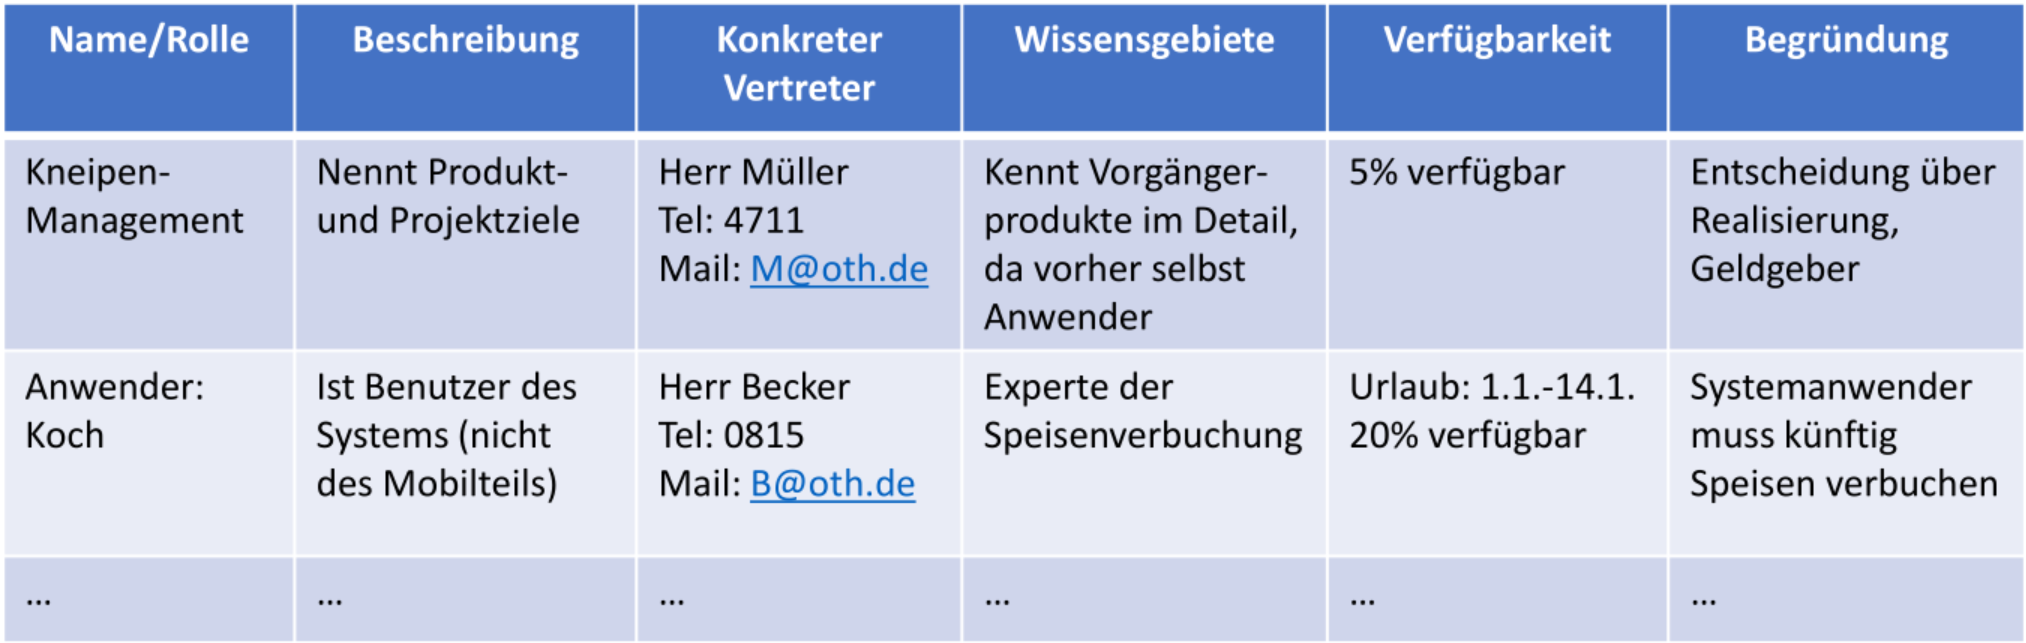
\includegraphics[width=1\textwidth]{Stakeholder-00}
    \caption{Stakeholderliste}
    \label{fig:Stakeholder-00}
\end{figure}

$ \rightarrow $ Übersehen von Stakeholdern kann zu unvollständigen Anforderungen führen

\subsubsection*{Checkliste zum Finden von Stakeholdern}

\begin{itemize}
    \item Wartungs- und Servicepersonal
    \begin{itemize}
        \item Wartung und Service muss unkompliziert und zügig durchzuführen sein
        \item Wichtig bei hohen Stückzahlen
    \end{itemize}
    \item Produktbeseitiger
    \begin{itemize}
        \item Wichtig, wenn ausgeliefertes Produkt nicht nur Software umfasst, Frage der Beseitigung (z.B. Umweltschutz), kann enormen Einfluss auf Zielsetzung von Produktentwicklung haben
    \end{itemize}
    \item Schulungs- und Trainingspersonal
    \begin{itemize}
        \item Liefern konkrete Anforderungen zu Bedienbarkeit, Vermittelbarkeit, Hilfesystem, Dokumentation, Erlernbarkeit
    \end{itemize}
    \item Marketing und Vertriebsabteilung
    \begin{itemize}
        \item Als interne Repräsentanten externer Kundenwünsche und Marktentwicklung
    \end{itemize}
    \item Systemschützer
    \begin{itemize}
        \item Stellen Anforderungen zum Schutz vor Fehlverhalten von Stakeholdern
    \end{itemize}
    \item Standards und Gesetze
    \begin{itemize}
        \item Vorhandene und zukünftige Standards/Gesetze berücksichtigen
    \end{itemize}
    \item Projekt- und Produktgegner
    \begin{itemize}
        \item Vor allem zu Beginn des Projekts möglichst mit einbeziehen, sonst drohen Konflikte
    \end{itemize}
    \item Kulturkreis
    \begin{itemize}
        \item Setzt Rahmenbedingungen, z.B. verwendete Symbolik, Begriffe, …
    \end{itemize}
    \item Meinungsführer und die öffentliche Meinung
    \begin{itemize}
        \item Beeinflussen oder schreiben Ziele vor, Zielmärkte berücksichtigen
    \end{itemize}
\end{itemize}


\subsection{Ermittlungstechniken}

\subsubsection*{Befragungstechniken}
\begin{itemize}
    \item \textbf{Interviews}: Direktes Gespräch zwischen Requirements Engineer und Stakeholder.
    \item \textbf{Fragebögen}: Standardisierte Fragen zur Sammlung von Anforderungen.
\end{itemize}

\subsubsection*{Dokumentengetrieben}
\begin{itemize}
    \item \textbf{Systemarchäologie}: Analyse der Dokumentation bestehender Systeme.
    \item \textbf{Perspektivenbasiertes Lesen}: Untersuchen von Dokumenten aus verschiedenen Perspektiven.
    \item \textbf{Wiederverwendung}: Bereits erstellte Anforderungen nutzen.
\end{itemize}

\subsubsection*{Beobachtungstechniken}
\begin{itemize}
    \item \textbf{Feldbeobachtung}: Beobachtung des Stakeholders in dessen gewohnter Umgebung.
    \item \textbf{Apprenticing}: Requirements Engineer erlernt die Tätigkeit des Stakeholders.
\end{itemize}

\subsubsection*{Kreativitätstechniken}
\begin{itemize}
    \item \textbf{Brainstorming}: Ideenfindung in Gruppen.
    \item \textbf{Perspektivenwechsel}: Betrachtung des Problems aus verschiedenen Blickwinkeln.
\end{itemize}


\subsection{Anforderungen dokumentieren}

\subsubsection*{Benutzeranforderungen (Was? und Wofür?):}
\begin{itemize}
    \item Aussagen in natürlicher Sprache (Vorteile/Nachteile?)
    \item Einfache Diagramme (Vorteile/Nachteile?)
    \item Beschreiben Dienste, die System leisten soll
    \item Beschreiben Randbedingungen unter denen System betrieben wird
    \item Systembeschreibung aus Kundensicht \textbf{(→ Lastenheft)}
\end{itemize}

\subsubsection*{Systemanforderungen (Wie? und Womit?):}
\begin{itemize}
    \item Detaillierte Festlegung von Funktionen, Diensten und Beschränkungen
    \item Beschreibung, was implementiert werden soll
    \item Systembeschreibung aus technischer Sicht \textbf{(→ Pflichtenheft))}
\end{itemize}

\subsubsection{Lastenheft}
\begin{itemize}
    \item Wird von Auftraggeber erstellt
    \item Beschreibung des \textbf{“Was”} und \textbf{"Wofür”}
    \item “Grobes” Pflichtenheft
    \item Details werden bewusst offen gelassen
\end{itemize}

\subsubsection{Pflichtenheft}
\begin{itemize}
    \item Wird vom Auftragnehmer erstellt
    \item Beschreibung des \textbf{Wie} und \textbf{“Womit”}
    \item Zu lieferndes System wird detailliert
    \item Systembeschreibung aus technischer Sicht
\end{itemize}


\subsubsection*{Templates nach Balzert:}

\noindent
\begin{minipage}[t]{0.45\textwidth}
    \textbf{Lastenheft}
    \begin{enumerate}
        \item Vision und Ziele
        \item Rahmenbedingungen
        \item Kontext und Überblick
        \item Funktionale Anforderungen
        \item Qualitätsanforderungen
    \end{enumerate}
\end{minipage}
\hfill
\begin{minipage}[t]{0.45\textwidth}
    \textbf{Pflichtenheft}
    \begin{enumerate}
        \item Vision und Ziele
        \item Rahmenbedingungen
        \item Kontext und Überblick
        \item Funktionale Anforderungen
        \item Qualitätsanforderungen
        \item Abnahmekriterien
        \item Subsystemstruktur (optional)
        \item Glossar
    \end{enumerate}
\end{minipage}

\vspace{2em}

\textit{→ das Pflichtenheft ist eine Verfeinerung des Lastenheftes}






\subsection{Anforderungen prüfen und abstimmen}

\subsubsection*{Prüfung}
\begin{itemize}
    \item \textbf{Inspektionen}: Systematische Überprüfung der Anforderungen.
    \item \textbf{Reviews}: Überprüfung durch Stakeholder und Fachexperten.
    \item \textbf{Walkthroughs}: Schritt-für-Schritt-Durchgang der Anforderungen.
\end{itemize}

\subsubsection*{Validierung}
\begin{itemize}
    \item Überprüfung jeder Anforderung gegen Visionen und Ziele.
    \item Stakeholder-Review und formale Abnahme.
\end{itemize}

\newpage


\subsection{Kano-Modell}

\begin{enumerate}
    \item Basis-Merkmale:
    \begin{itemize}
        \item Grundlegend, Kunden merken es bei Nichterfüllung (implizite Erwartungen)
        \item Nichterfüllung führt zu Unzufriedenheit, Erfüllung führt nicht zu Zufriedenheit
        \item Geringe Nutzensteigerung gegenüber Wettbewerbern
        \item Beispiel Auto: Sicherheit, Rostschutz
    \end{itemize}
    \item Leistungs-Merkmale:
    \begin{itemize}
        \item Kunden bewusst, beseitigen Unzufriedenheit oder schaffen Zufriedenheit
        \item Beispiel Auto: Fahreigenschaften, Beschleunigung, Lebensdauer, Verbrauch
    \end{itemize}
    \item Begeisterungs-Merkmale:
    \begin{itemize}
        \item Nutzen stiftend, unerwartet, zeichnen Produkt aus, rufen Begeisterung hervor
        \item Kleine Leistungssteigerung, hoher Nutzen
        \item Beispiel Auto: Sonderausstattung, besonderes Design, Hybridtechnologie
    \end{itemize}
    \item Unerhebliche Merkmale:
    \begin{itemize}
        \item Ohne Belang für Kunden, stiften keine Zufriedenheit, führen nicht zu Unzufriedenheit
        \item Beispiel Auto: Automatikgetriebe, Schiebedach (je nach Kundengruppe)
    \end{itemize}
    \item Rückweisungs-Merkmale:
    \begin{itemize}
        \item Führen bei Vorhandensein zu Unzufriedenheit, bei Fehlen keine Zufriedenheit
        \item Beispiel Auto: Rostflecken, abgelaufener TÜV
    \end{itemize}
\end{enumerate}

\vspace{2em}

\begin{figure}[h]
    \centering
    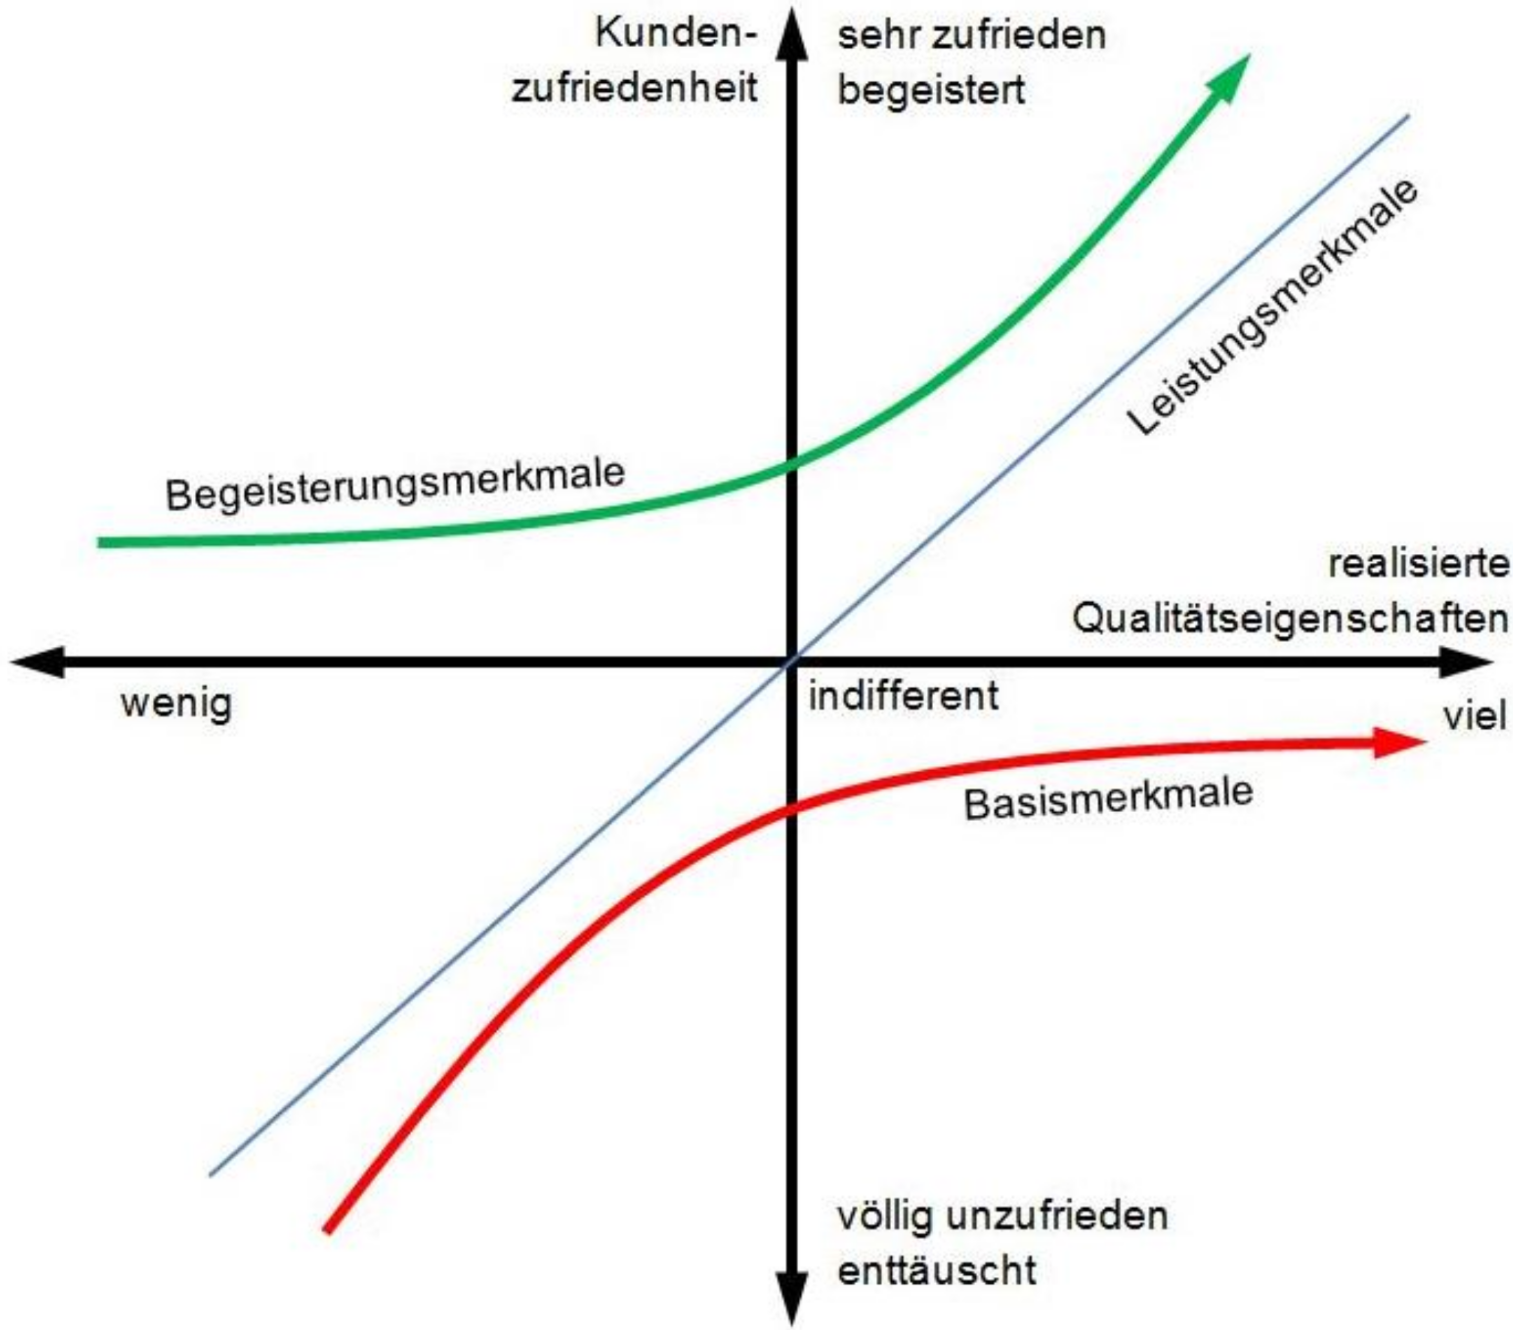
\includegraphics[width=0.5\textwidth]{Kano-00.png}
    \caption{Veranschaulichung des Kano-Modells}
    \label{fig:Kano-00}
\end{figure}

\newpage


Kano Modelle werden auf Basis von Kunden Befragungen ausgefüllt!

Hier ein Beispiel eines Kano Modells für intelligentes Krankenbett:

\vspace{1em}

\begin{figure}[h]
    \centering
    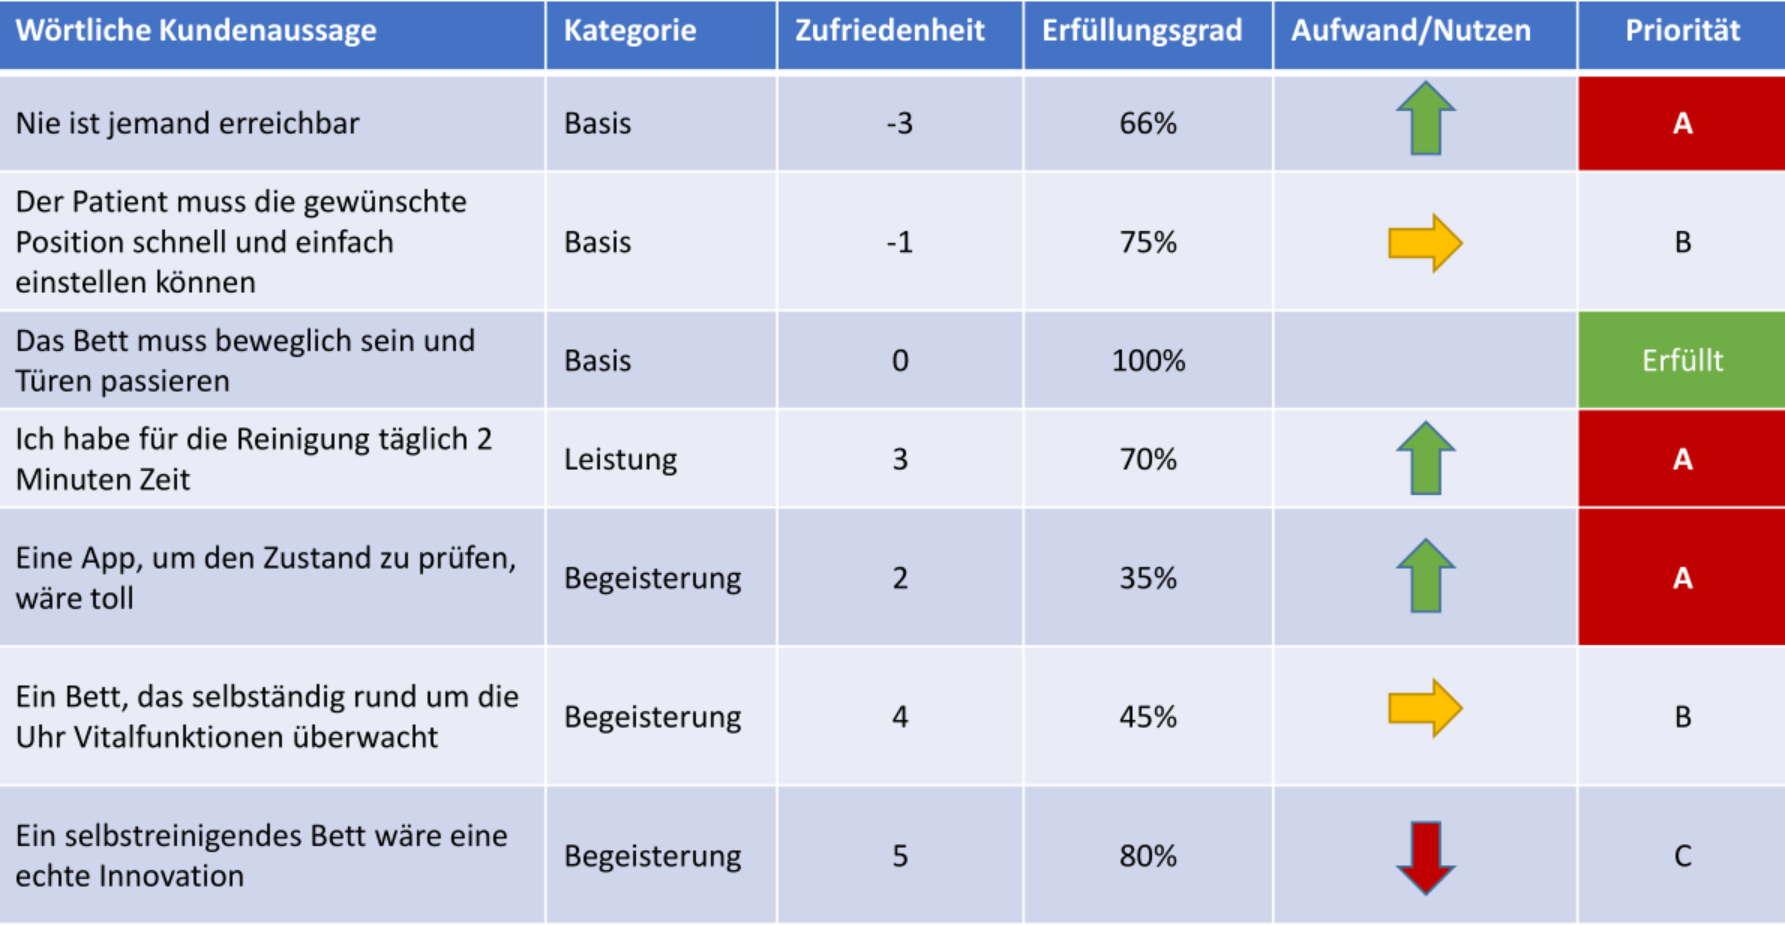
\includegraphics[width=0.8\textwidth]{Kano-01.png}
    \caption{Beispiel für Kano-Modell Tabelle}
    \label{fig:Kano-01}
\end{figure}


\begin{figure}[h]
    \centering
    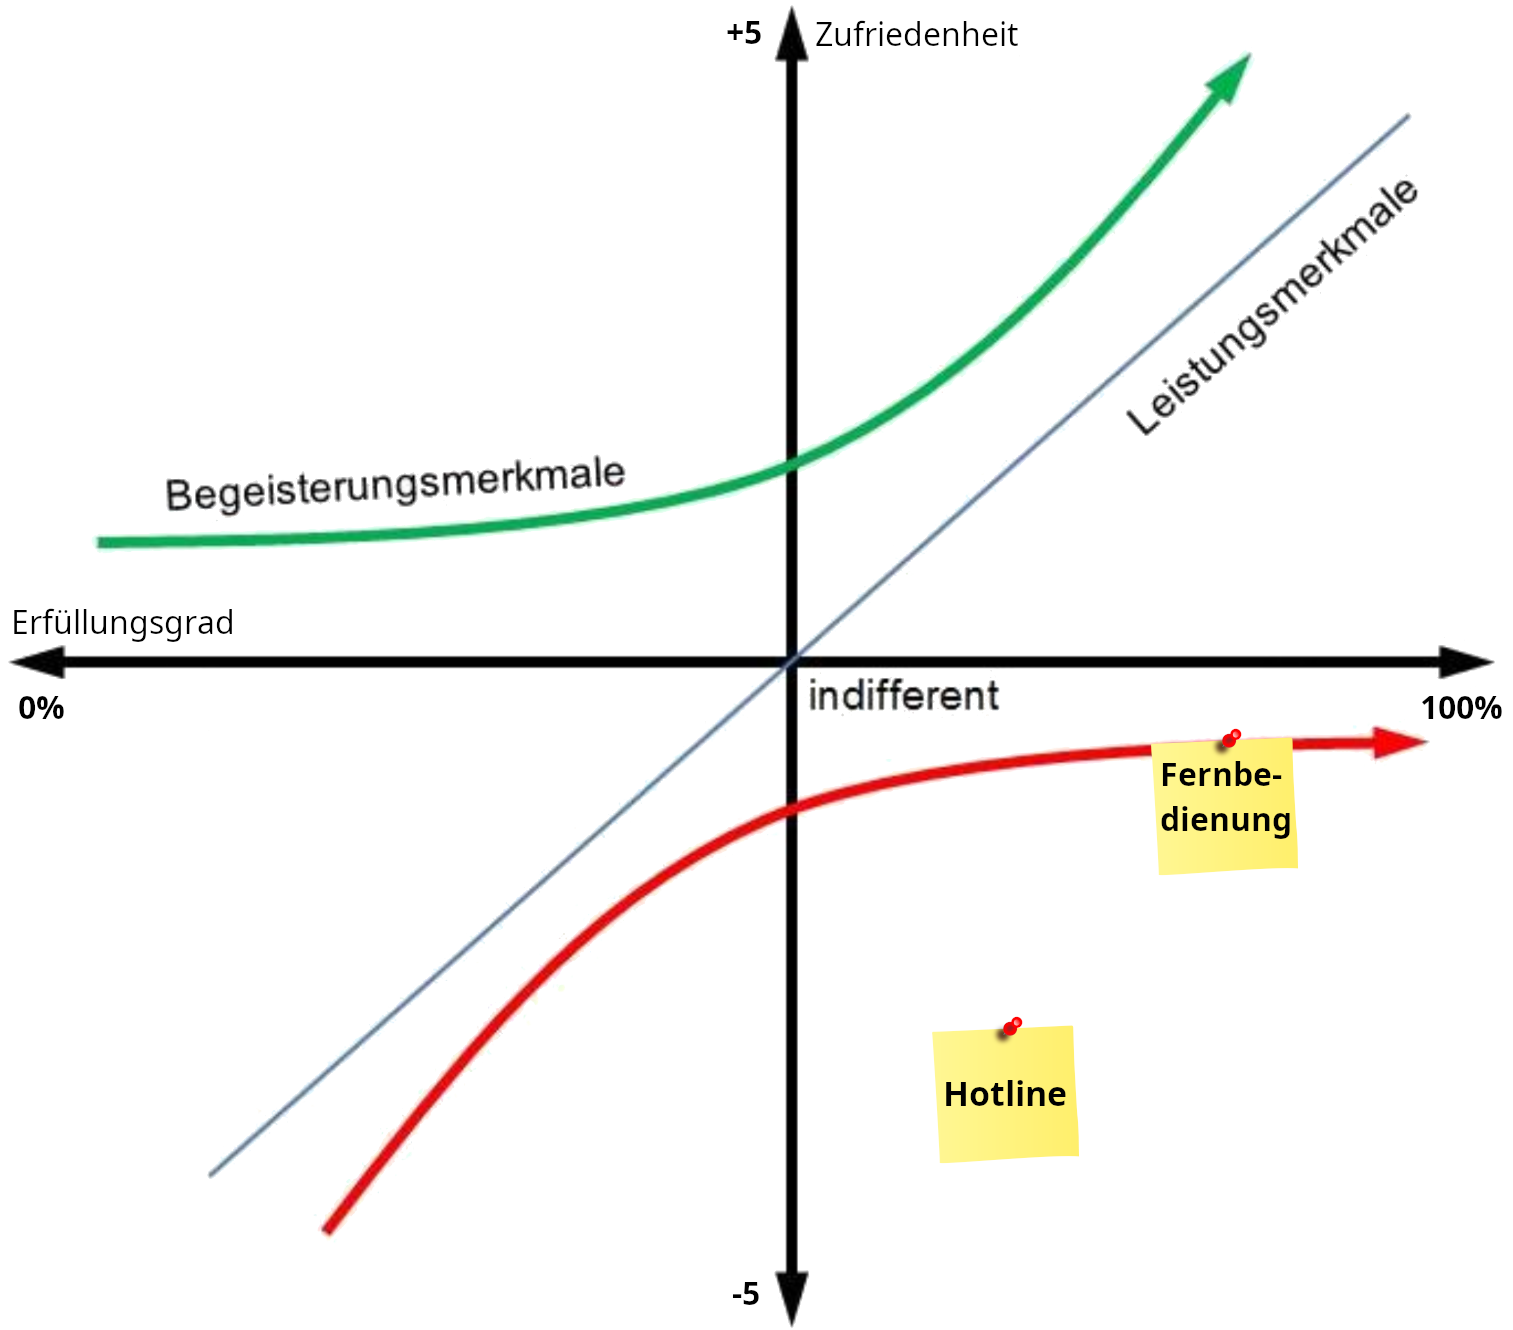
\includegraphics[width=0.5\textwidth]{Kano-02.png}
    \caption{Beispiel für Kano-Modell Graph}
    \label{fig:Kano-02}
\end{figure}

\vspace{2em}

\noindent \sloppy Die nicht erreichbare Hotline zum Beispiel, wird von den Kunden als -3 in der Zufriedenheit und 66\% im Erfüllungsgrad gewertet.
Auf dem Graphen ist dieses Merkmal unter der Basismerkmal Kurve und somit sehr schlecht.\\
Dadurch ist der Aufwand/Nutzen hoch und die Priorität 'A'.

\newpage



\subsection{Best practices}

\begin{itemize}
    \item Kunden und Benutzer einbinden
    \item Alle möglichen RE-Quellen identifizieren und konsultieren
    \item Erfahrene Projektmanager und Teammitglieder einsetzen
    \item 15 – 30 \% der Ressourcen für RE vorsehen
    \item Anforderungsschablonen und Beispiele zur Verfügung stellen
    \item Gute Beziehungen zu allen Beteiligten und Betroffenen herstellen
    \item Anforderungen priorisieren
    \item Ergänzende Modelle gemeinsam mit Prototypen entwickeln
    \item Eine Nachverfolgungsmatrix pflegen
    \item Peer Reviews durch Benutzer, Szenarien und Walk-Throughs zur Validierung und Verifizierung der Anforderungen durchführen
\end{itemize}



\subsection{Erfassung von Anforderungen}

\subsubsection{Requirements Analysis}

\begin{enumerate}
    \item Erfassung der Systemaufgaben mit \textbf{Use Cases}
    \item Beschreibung der Aufgaben mit \textbf{Aktivitätsdiagrammen}
    \item (optional) Formalisierung der Beschreibungen in \textbf{Anforderungen}
    \item Aufbau eines tieferen Verständnisses durch \textbf{Klassenmodellierung} und \textbf{Sequenzdiagramme} (Grobdesign)
\end{enumerate}

\vspace{1em}

$ \rightarrow $ \textbf{Was} sind die Hauptaufgaben des Systems?

$ \rightarrow $ \textbf{Wer} ist an den Aufgaben beteiligt?

$ \rightarrow $ \textbf{Welche Schritte} gehören zur Aufgabenerfüllung?

\newpage



\newpage


\section{Objektorientierte Analyse (OOA)} % --- Objektorientierte Analyse (OOA) ------------------------------------------------------------------------------------


\subsection{Kontext-Diagramme}

\textbf{Früh in Analysephase:} Systemkontext erfassen und dokumentieren

\begin{figure}[h]
    \centering
    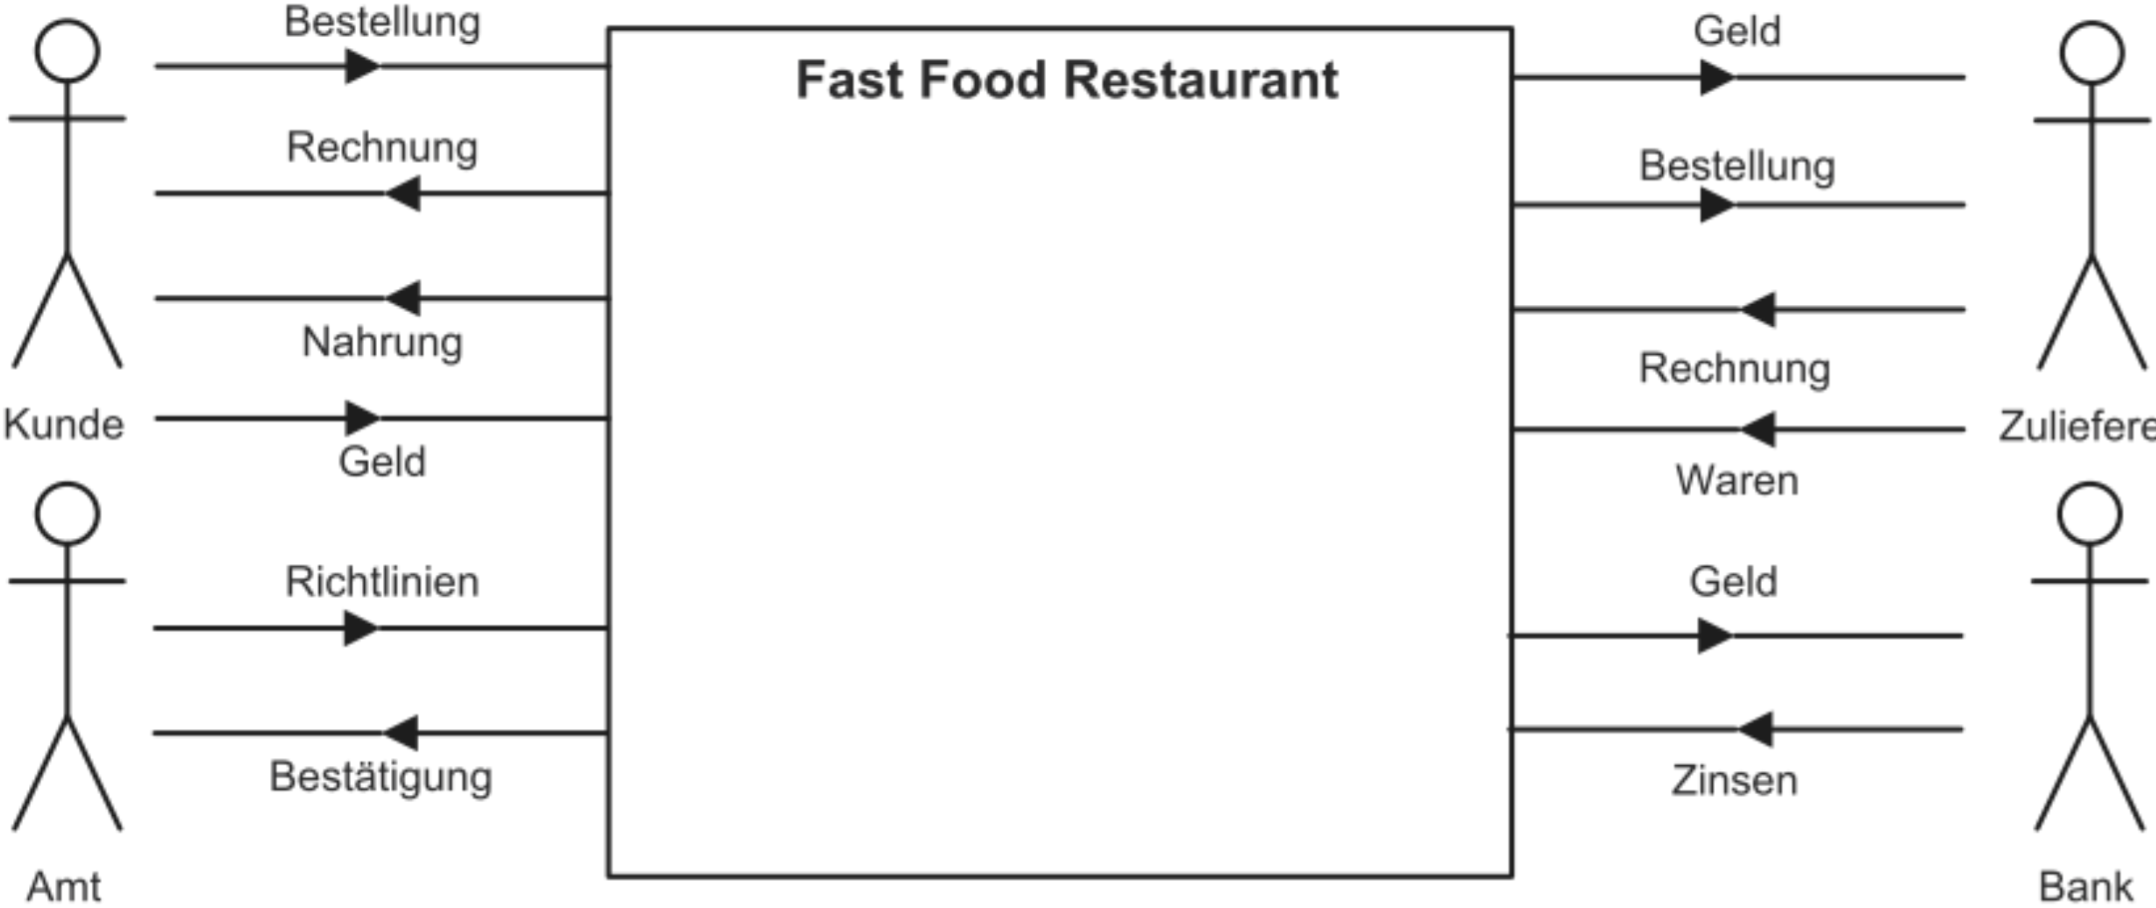
\includegraphics[width=0.75\textwidth]{KontextDiagramm-00.png}
    \caption{Biespiel eines Kontext Diagramm}
    \label{fig:KontextDiagramm-00}
\end{figure}

\newpage

\section{UML und Diagrammtypen}


\begin{figure}[h]
    \centering
    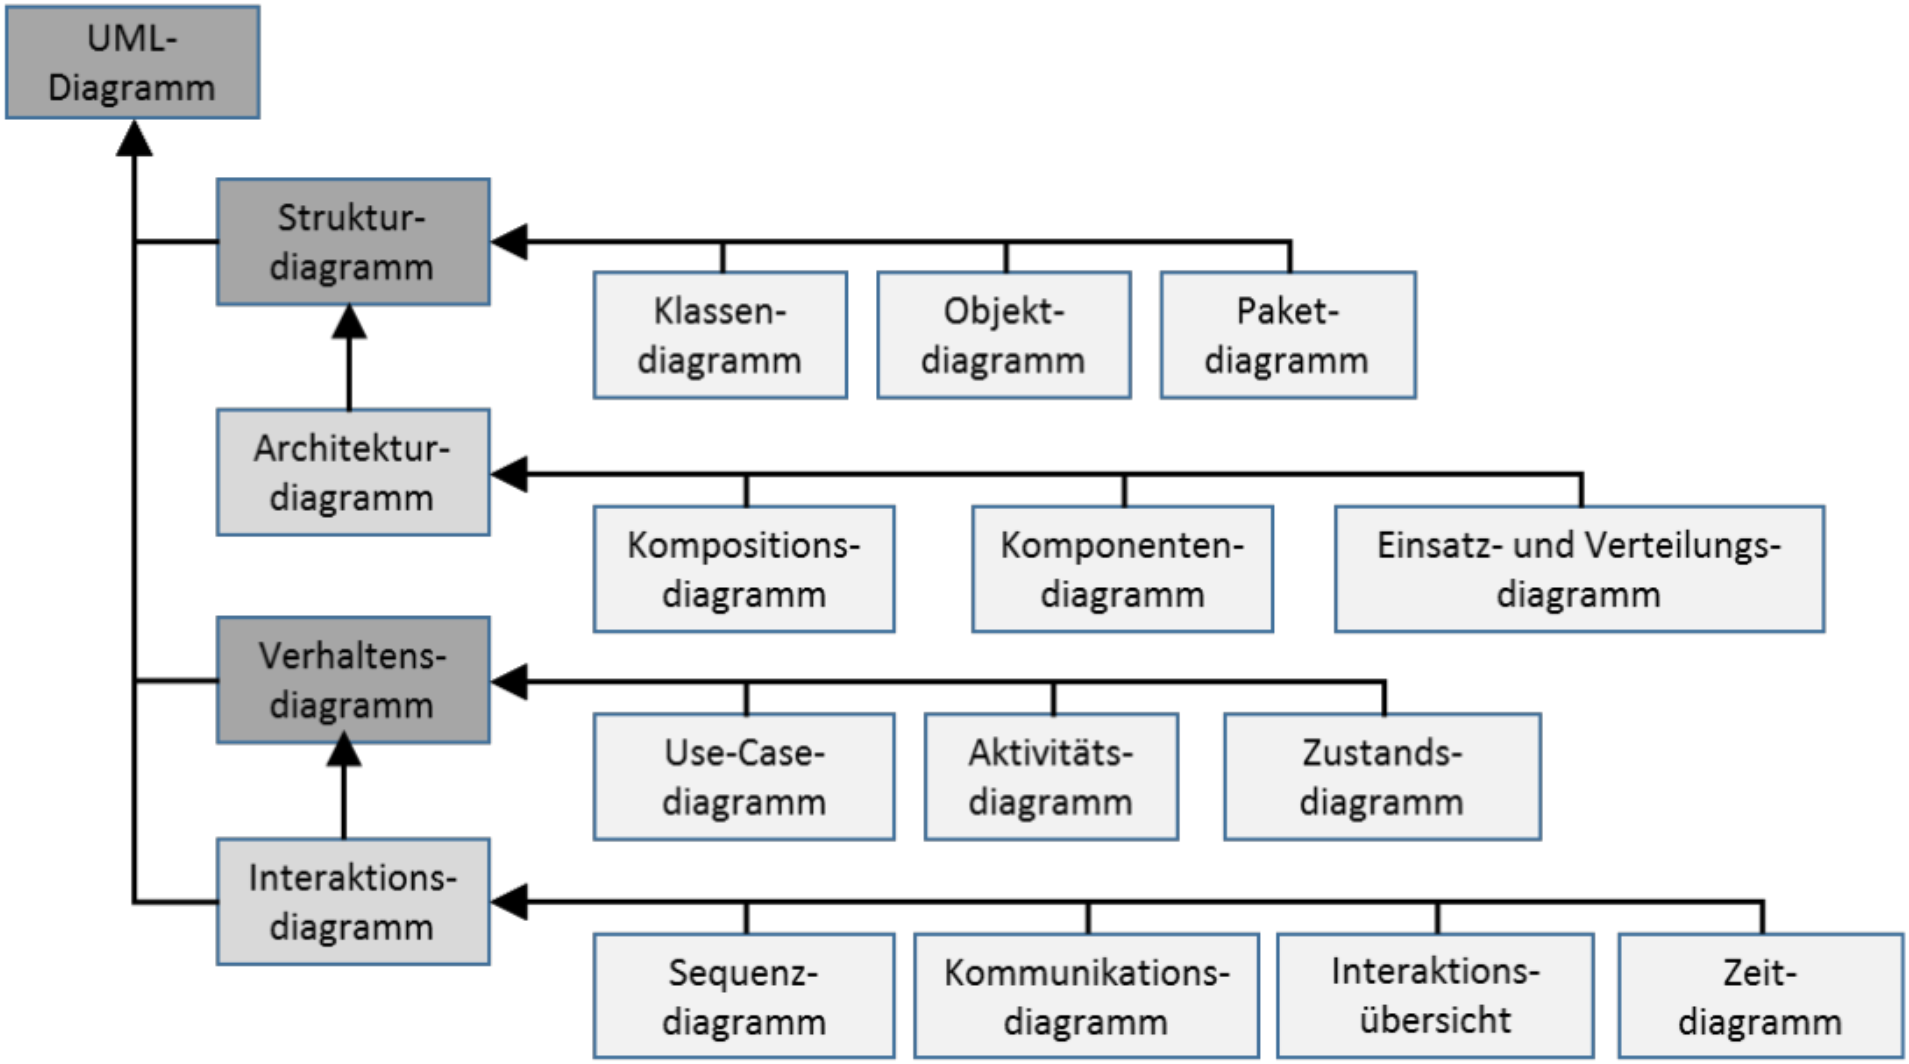
\includegraphics[width=0.75\textwidth]{UML-00.png}
    \caption{UML-Diagramme}
    \label{fig:UML-00}
\end{figure}


\vspace{5em}


\subsection{Use-Case-Diagramme}


\noindent \textbf{Ziel und Definition:} Spezifiziert Sequenz von Aktionen einschließlich möglicher Varianten, die das System in Interaktion mit Akteuren auslöst. Es ist als Black-Box zu verstehen!

\vspace{1em}

\noindent\textbf{Erfragung des “WAS”?}
\begin{itemize}
    \item Was sind die Hauptaufgaben des Systems?
    \item Wer ist beteiligt?
    \item Welche Schritte gehören zur Aufgabenerfüllung?
    \item Aufgaben als Use Cases, Beteiligte als Akteure.
\end{itemize}

\vspace{1em}

\noindent\textbf{Struktur eines Use Cases:}
\begin{itemize}
    \item Titel, Kurzbeschreibung, Aktoren, Vorbedingungen, Ablauf, Auswirkungen, Anmerkungen.
\end{itemize}

\vspace{1em}

\noindent\textbf{Akteure:} Ein Akteur ist ein Objekt der Systemumgebung, das mit dem System interagiert und Use Cases auslösen kann. Akteure können Personen, externe Geräte oder Nachbarsysteme sein.

\newpage

\subsubsection{Standardelemente}

\begin{figure}[ht]
    \centering
    \begin{minipage}[t]{0.30\textwidth}
        \centering Aktor \\
        \vspace{1em}
        \centering 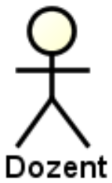
\includegraphics[width=0.2\textwidth]{UseCase-00.png}
    \end{minipage}
    \centering
    \begin{minipage}[t]{0.30\textwidth}
        \centering Use Case \\
        \vspace{1em}
        \centering 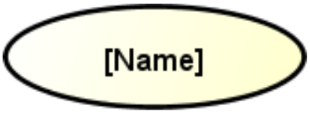
\includegraphics[width=0.5\textwidth]{UseCase-01.png}
    \end{minipage}
    \centering
    \begin{minipage}[t]{0.30\textwidth}
        \centering Systemgrenze \\
        \vspace{1em}
        \centering 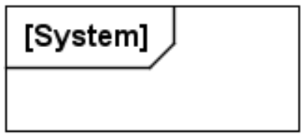
\includegraphics[width=0.5\textwidth]{UseCase-02.png}
    \end{minipage}
\end{figure}

\vspace{1em}

\begin{figure}[ht]
    \centering
    \begin{minipage}[t]{0.45\textwidth}
        \centering 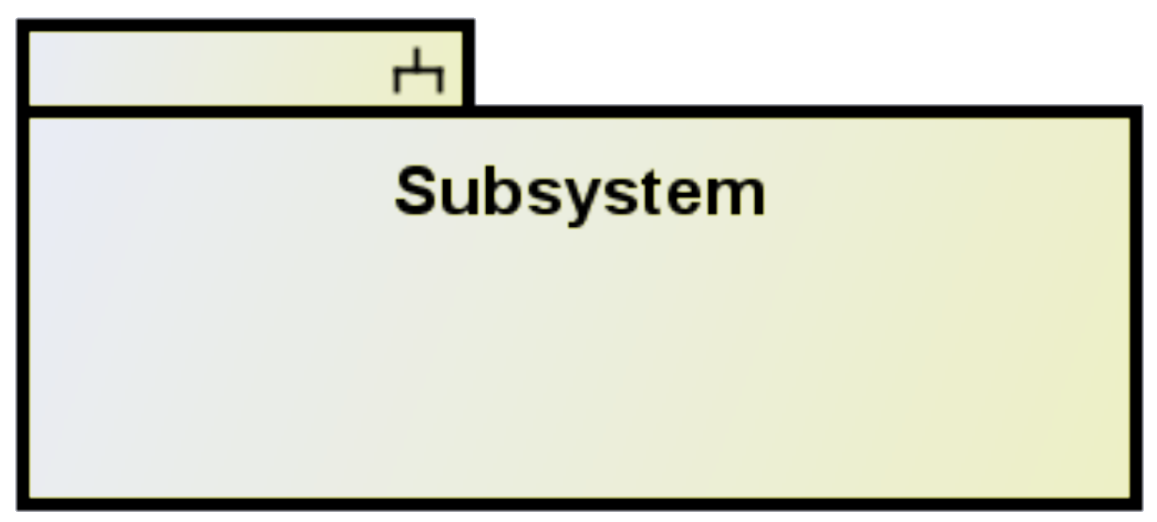
\includegraphics[width=0.4\textwidth]{UseCase-08.png} \\
        \vspace{1em}
        \centering Subsystem
    \end{minipage}
    \centering
    \begin{minipage}[t]{0.45\textwidth}
        \centering 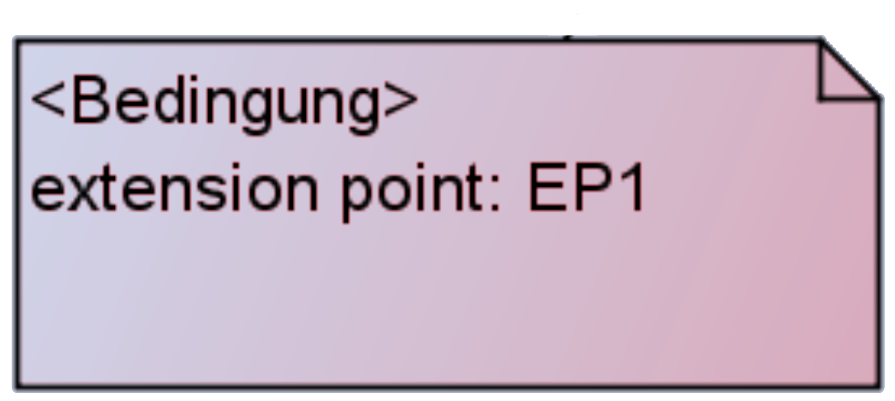
\includegraphics[width=0.4\textwidth]{UseCase-09.png} \\
        \vspace{1em}
        \centering Bedingung
    \end{minipage}
\end{figure}

\vspace{1em}

\begin{figure}[ht]
    \centering
    \begin{minipage}[t]{0.45\textwidth}
        \centering 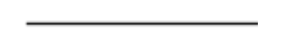
\includegraphics[width=0.4\textwidth]{UseCase-03.png} \\
        \vspace{1em}
        \centering Kommunikationsbeziehung zwischen Aktoren und Use Cases
    \end{minipage}
    \centering
    \begin{minipage}[t]{0.45\textwidth}
        \centering 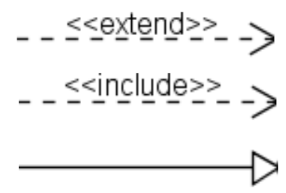
\includegraphics[width=0.4\textwidth]{UseCase-04.png} \\
        \vspace{1em}
        \centering Beziehung zwischen \\ Anwendungsfällen
    \end{minipage}
\end{figure}





\newpage

\subsubsection*{Beispiele}
\vspace{1em}

\centering Vollständiges Use-Case-Diagramm \\
\begin{figure}[h]
    \centering
    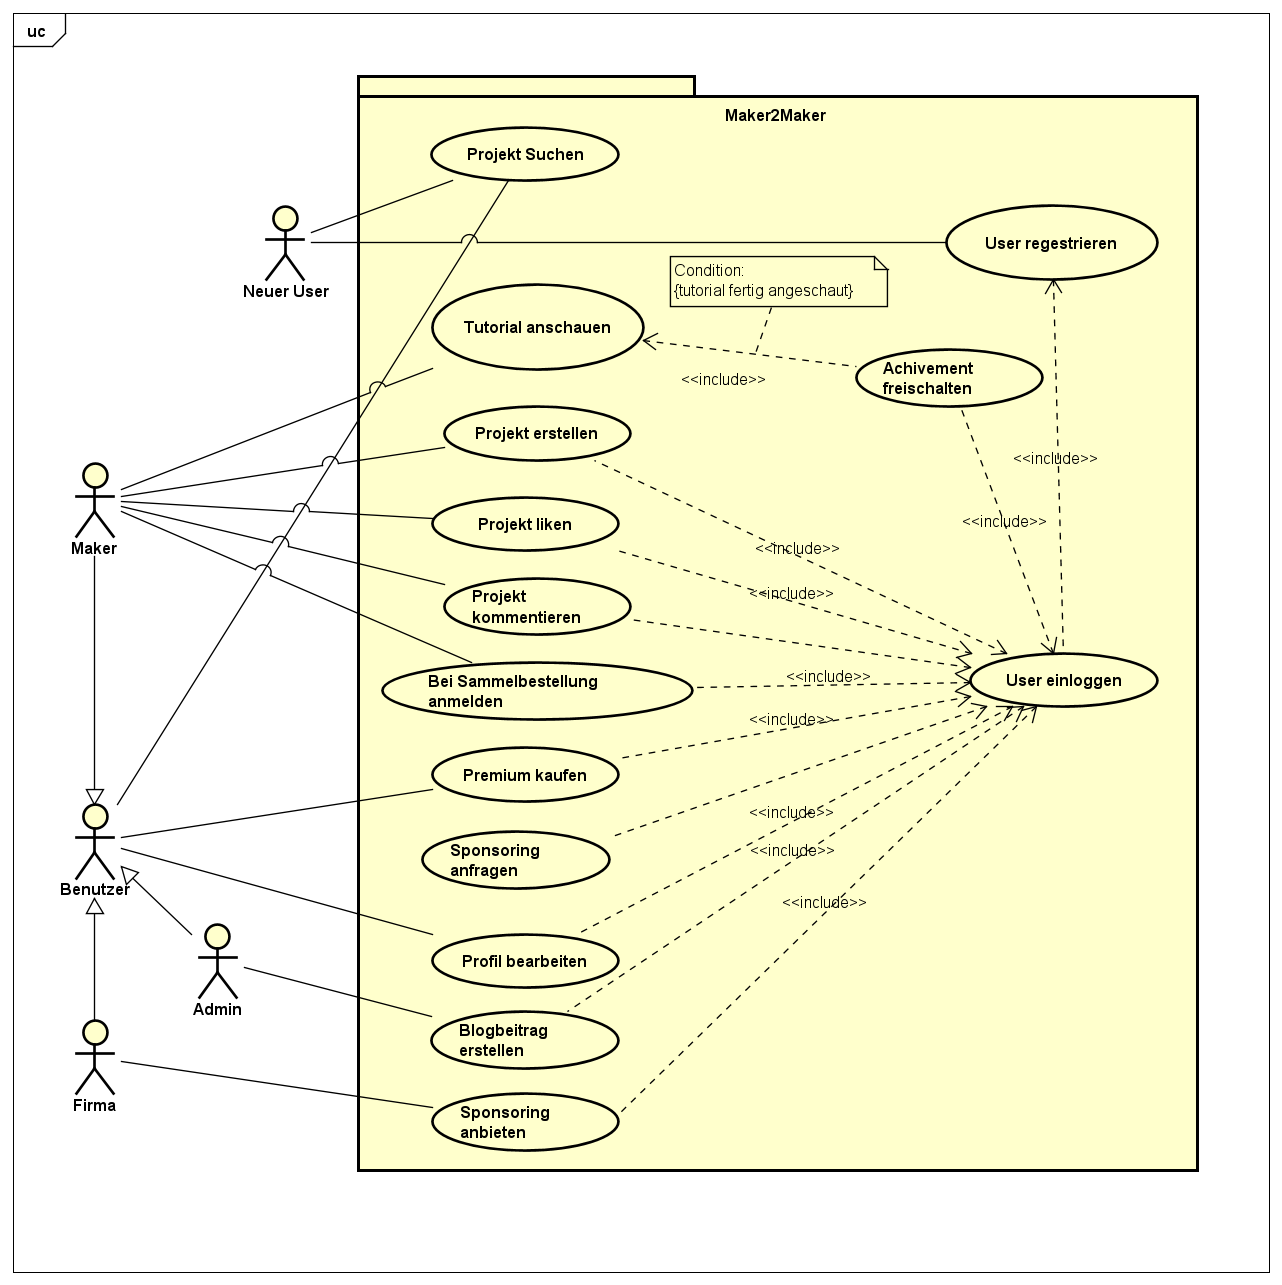
\includegraphics[width=0.70\textwidth]{UseCase-07.png}
    \label{fig:UseCase-07}
\end{figure}

\vspace{1em}

\centering Use-Case-Diagramm mit Subsystem \\
\begin{figure}[h]
    \centering
    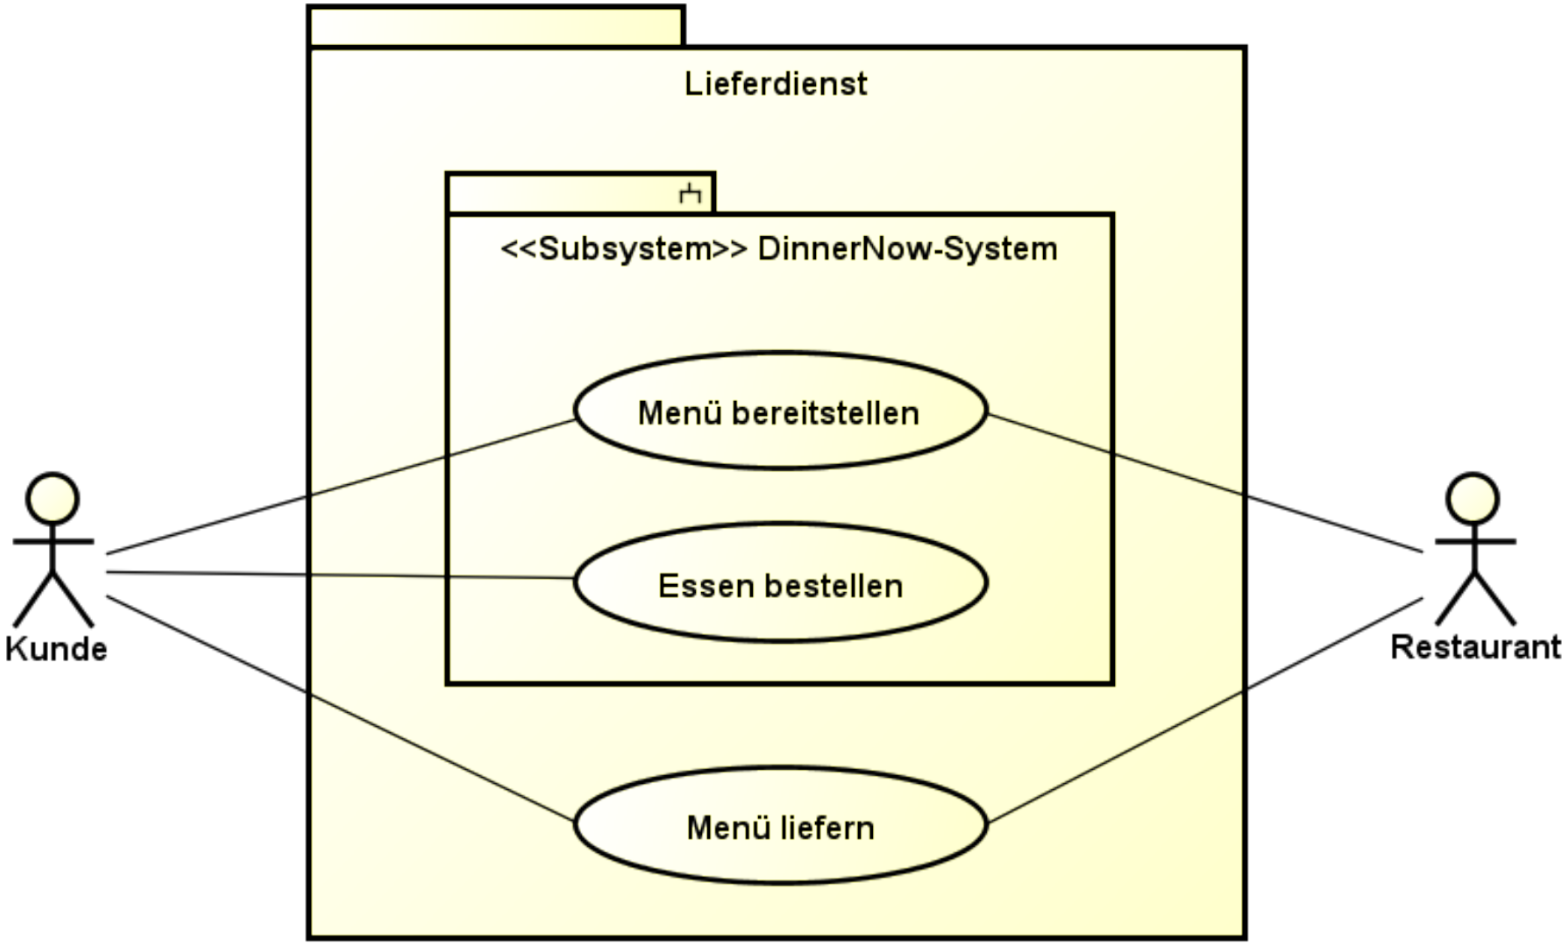
\includegraphics[width=0.5\textwidth]{UseCase-10.png}
    \label{fig:UseCase-10}
\end{figure}

\newpage



\raggedright \subsubsection{<<include>>}

\begin{itemize}
    \item Visualisiert, dass Use Case A das Verhalten von Use Case B importiert
\end{itemize}

\begin{figure}[h]
    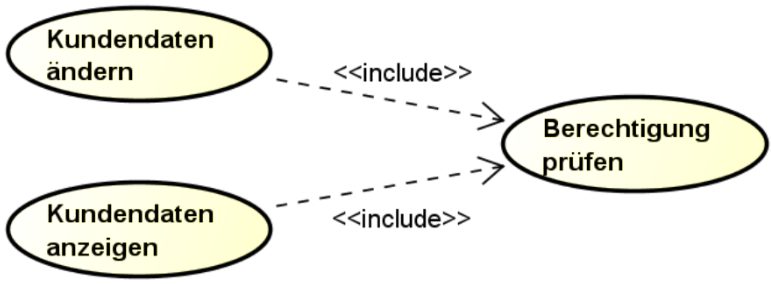
\includegraphics[width=0.3\textwidth]{UseCase-11.png}
    \label{fig:UseCase-11}
\end{figure}

\raggedright \subsubsection{<<extend>>}

\begin{itemize}
    \item Verhalten von Use-Case 2 kann durch Use-Case 1 erweitert werden (muss aber nicht)
    \item Ein Use Case darf mehrere Erweiterungspunkte besitzen
\end{itemize}

\begin{figure}[h]
    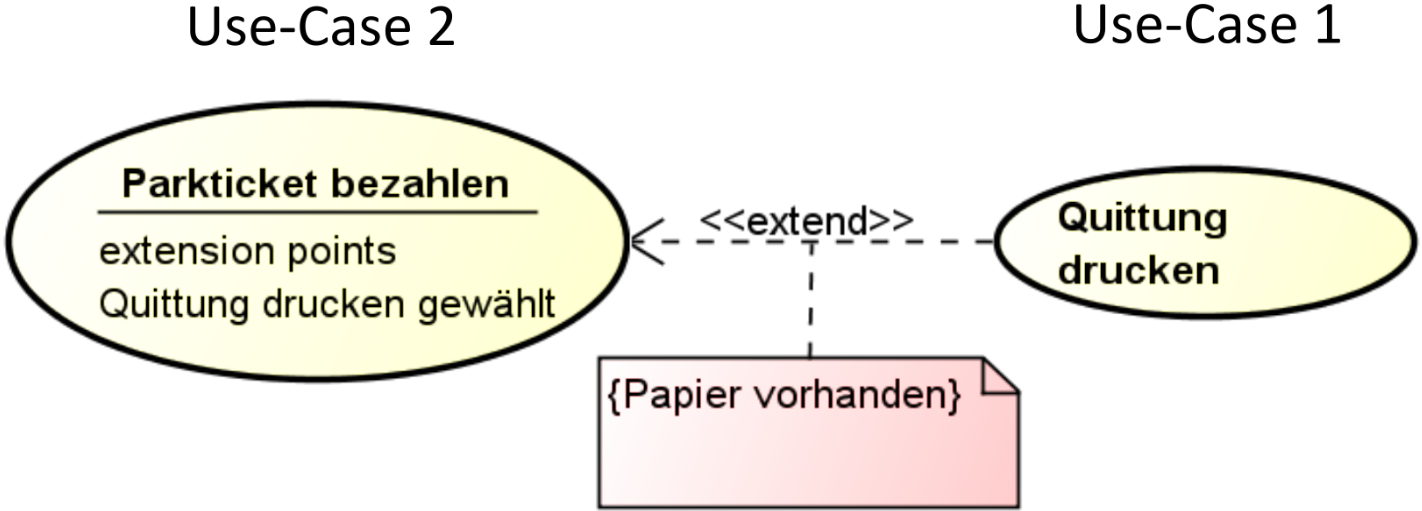
\includegraphics[width=0.3\textwidth]{UseCase-12.png}
    \label{fig:UseCase-12}
\end{figure}

\textbf{Achtung:} Pfeil weist in die Richtung des Use-Cases, der erweitert werden soll


\subsection{Use-Case-Definitionen}

\subsubsection*{Beispiele}

\begin{figure}[ht]
    \centering
    \begin{minipage}[t]{0.45\textwidth}
        \centering 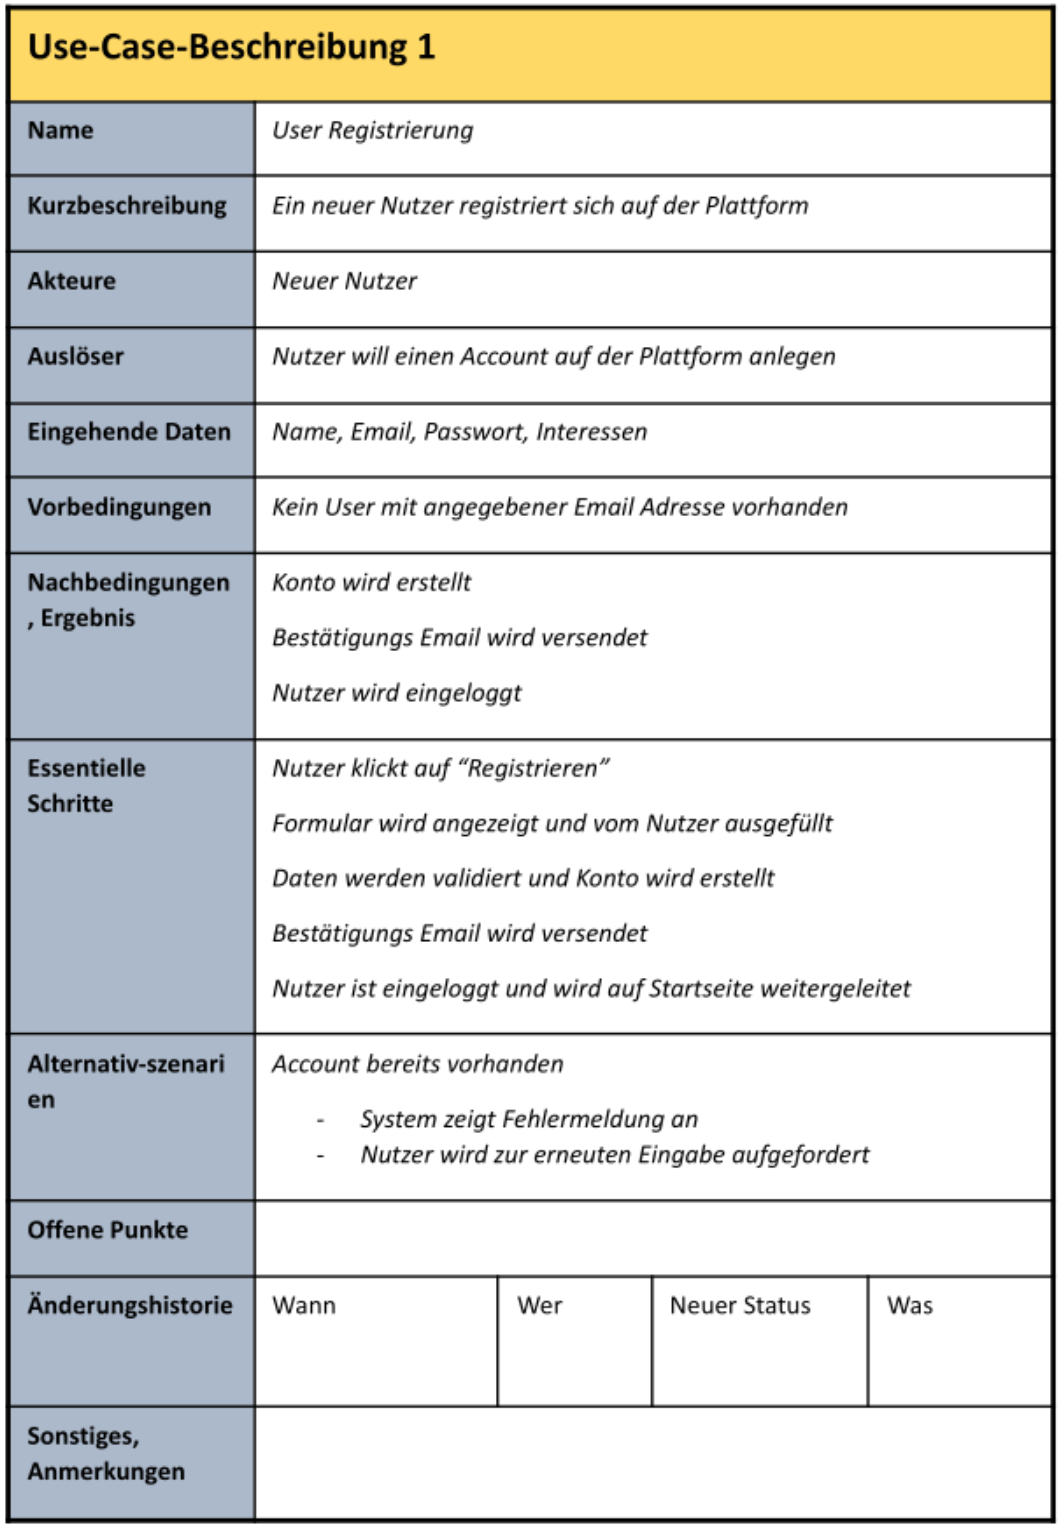
\includegraphics[width=0.9\textwidth]{UseCase-13.png} \\
    \end{minipage}
    \centering
    \begin{minipage}[t]{0.45\textwidth}
        \centering 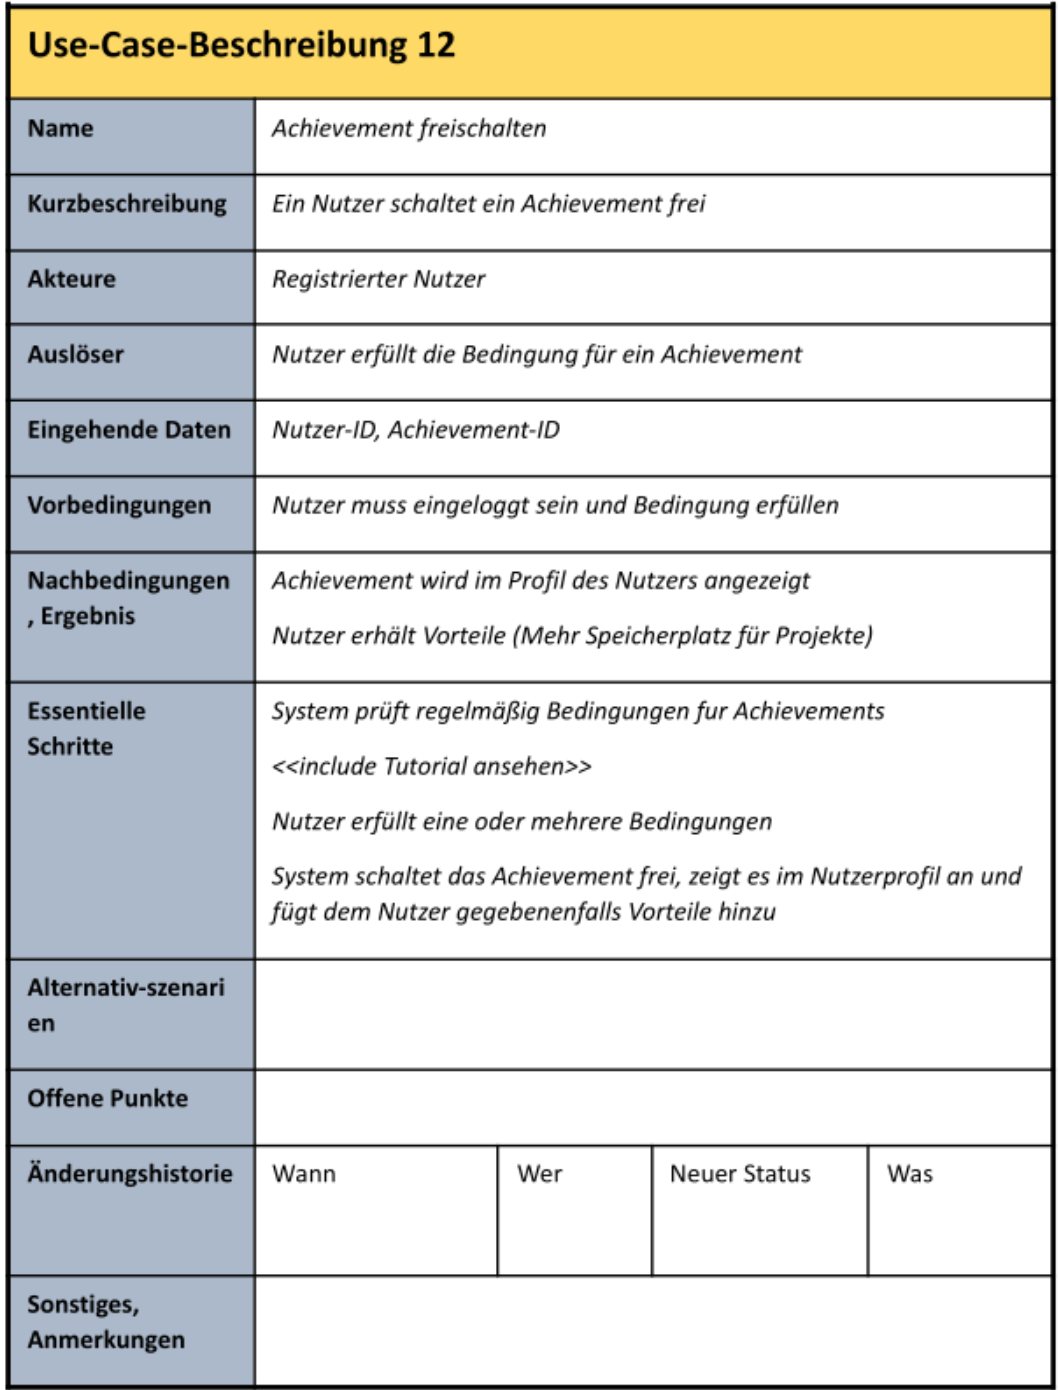
\includegraphics[width=0.9\textwidth]{UseCase-14.png} \\
        \vspace{1em}
        \centering mit <<include>>
    \end{minipage}
\end{figure}




\section{Objektorientiertes Design (OOD)} % --- Objektorientiertes Design (OOD) ------------------------------------------------------------------------------------


\section{Entwurf und Implementierung} % --- Entwurf und Implementierung ------------------------------------------------------------------------------------


\section{Design Patterns} % --- Design Patterns ------------------------------------------------------------------------------------


\section{Testen} % --- Testen ------------------------------------------------------------------------------------


\section{Vorgehensmodelle} % --- Vorgehensmodelle ------------------------------------------------------------------------------------




\end{document}